% Options for packages loaded elsewhere
\PassOptionsToPackage{unicode}{hyperref}
\PassOptionsToPackage{hyphens}{url}
\PassOptionsToPackage{dvipsnames,svgnames*,x11names*}{xcolor}
%
\documentclass[
]{article}
\usepackage{lmodern}
\usepackage{amsmath}
\usepackage{ifxetex,ifluatex}
\ifnum 0\ifxetex 1\fi\ifluatex 1\fi=0 % if pdftex
  \usepackage[T1]{fontenc}
  \usepackage[utf8]{inputenc}
  \usepackage{textcomp} % provide euro and other symbols
  \usepackage{amssymb}
\else % if luatex or xetex
  \usepackage{unicode-math}
  \defaultfontfeatures{Scale=MatchLowercase}
  \defaultfontfeatures[\rmfamily]{Ligatures=TeX,Scale=1}
  \setmainfont[]{lm}
\fi
% Use upquote if available, for straight quotes in verbatim environments
\IfFileExists{upquote.sty}{\usepackage{upquote}}{}
\IfFileExists{microtype.sty}{% use microtype if available
  \usepackage[]{microtype}
  \UseMicrotypeSet[protrusion]{basicmath} % disable protrusion for tt fonts
}{}
\makeatletter
\@ifundefined{KOMAClassName}{% if non-KOMA class
  \IfFileExists{parskip.sty}{%
    \usepackage{parskip}
  }{% else
    \setlength{\parindent}{0pt}
    \setlength{\parskip}{6pt plus 2pt minus 1pt}}
}{% if KOMA class
  \KOMAoptions{parskip=half}}
\makeatother
\usepackage{xcolor}
\IfFileExists{xurl.sty}{\usepackage{xurl}}{} % add URL line breaks if available
\IfFileExists{bookmark.sty}{\usepackage{bookmark}}{\usepackage{hyperref}}
\hypersetup{
  pdftitle={Farmers advised by both public and private extension systems are more likely to adopt climate-smart agriculture in West Africa},
  colorlinks=true,
  linkcolor=Maroon,
  filecolor=Maroon,
  citecolor=Blue,
  urlcolor=Blue,
  pdfcreator={LaTeX via pandoc}}
\urlstyle{same} % disable monospaced font for URLs
\usepackage{longtable,booktabs}
\usepackage{calc} % for calculating minipage widths
% Correct order of tables after \paragraph or \subparagraph
\usepackage{etoolbox}
\makeatletter
\patchcmd\longtable{\par}{\if@noskipsec\mbox{}\fi\par}{}{}
\makeatother
% Allow footnotes in longtable head/foot
\IfFileExists{footnotehyper.sty}{\usepackage{footnotehyper}}{\usepackage{footnote}}
\makesavenoteenv{longtable}
\setlength{\emergencystretch}{3em} % prevent overfull lines
\providecommand{\tightlist}{%
  \setlength{\itemsep}{0pt}\setlength{\parskip}{0pt}}
\setcounter{secnumdepth}{5}
\usepackage[margin=2.8cm]{geometry}
\renewcommand{\contentsname}{Table of Contents}
\usepackage{enumitem}
\usepackage{pifont}
\renewcommand{\labelitemi}{$\rightarrow$}
\usepackage{tocloft}
\renewcommand\cftsecleader{\cftdotfill{\cftdotsep}}
\usepackage{hyperref}
\hypersetup{linkcolor = blue}
\usepackage{hanging}
\usepackage[T1]{fontenc}
\usepackage{graphicx}
\usepackage{booktabs,threeparttablex}
\usepackage{multirow}
\usepackage{caption}
\usepackage{pdflscape}
\usepackage{fvextra}
\DefineVerbatimEnvironment{Highlighting}{Verbatim}{breaklines,commandchars=\\\{\}}
\usepackage{lmodern}
\usepackage{nimbusmono}
\renewcommand{\thetable}{SM\arabic{table}}
\renewcommand{\thefigure}{SM\arabic{figure}}
\setlength{\cfttabnumwidth}{1cm}
\usepackage{fouriernc}
\usepackage{booktabs}
\usepackage{longtable}
\usepackage{array}
\usepackage{multirow}
\usepackage{wrapfig}
\usepackage{float}
\usepackage{colortbl}
\usepackage{pdflscape}
\usepackage{tabu}
\usepackage{threeparttable}
\usepackage{threeparttablex}
\usepackage[normalem]{ulem}
\usepackage{makecell}
\usepackage{xcolor}
\ifluatex
  \usepackage{selnolig}  % disable illegal ligatures
\fi

\title{Farmers advised by both public and private extension systems are more likely to adopt climate-smart agriculture in West Africa}
\usepackage{etoolbox}
\makeatletter
\providecommand{\subtitle}[1]{% add subtitle to \maketitle
  \apptocmd{\@title}{\par {\large #1 \par}}{}{}
}
\makeatother
\subtitle{Supplementary Material}
\date{Last updated: 2023-12-02 10:07:48.162413}

\begin{document}
\maketitle

\newpage

\newpage
\listoftables
\listoffigures
\newpage

\begin{table}[ht]
\centering
\caption{Sample Size by Country and Year}
\begin{tabular}{@{}lccc@{}}
\toprule
Country & 2017 & 2018 & 2019 \\ 
\midrule
Ghana   &  900 &  540 &  506 \\
Mali    & 1350 &  900 &  840 \\
Nigeria & 2500 & 1600 & 1530 \\
\bottomrule
\end{tabular}

\label{tab:sample_size}
\end{table}

\begin{figure}[!htb]
  \centering

      \includegraphics[width=\textwidth]{descriptive_plot_interest_3.png}
  \caption{Descriptive plot: Distribution of extension systems by year}
\end{figure}

\clearpage

\begin{table}[]
\caption{Correlation between CSA practises by country}
\label{tab:my-table}
\resizebox{\textwidth}{!}{%
\begin{tabular}{llrrrrrr}
\hline
Variable1      & Variable2          & \multicolumn{1}{l}{Coefficient} & \multicolumn{1}{l}{Robust std. err.} & \multicolumn{1}{l}{Z} & \multicolumn{1}{l}{P \textgreater Z} & \multicolumn{2}{l}{{[}95\% conf. interval{]}} \\ \hline
\multicolumn{8}{l}{\cellcolor[HTML]{DBE8FF}Overall}                                                                                                                                                                         \\ \hline
Crop rotation  & Improved seeds     & -0.049                          & 0.048                                & -1.02                 & 0.31                                 & -0.143                & 0.045                 \\
Crop rotation  & Intercropping      & 0.348                           & 0.104                                & 3.33                  & 0.001                                & 0.143                 & 0.552                 \\
Crop rotation  & Organic fertilizer & 0.168                           & 0.084                                & 1.99                  & 0.046                                & 0.003                 & 0.332                 \\
Improved seeds & Intercropping      & -0.136                          & 0.041                                & -3.33                 & 0.001                                & -0.216                & -0.056                \\
Improved seeds & Organic fertilizer & 0.141                           & 0.079                                & 1.79                  & 0.074                                & -0.014                & 0.296                 \\
Intercropping  & Organic fertilizer & 0.294                           & 0.083                                & 3.55                  & 0                                    & 0.132                 & 0.457                 \\ \hline
\multicolumn{8}{l}{\cellcolor[HTML]{DBE8FF}Ghana}                                                                                                                                                                           \\ \hline
Crop rotation  & Improved seeds     & -0.043                          & 0.08                                 & -0.53                 & 0.595                                & -0.2                  & 0.114                 \\
Crop rotation  & Intercropping      & 0.029                           & 0.213                                & 0.14                  & 0.891                                & -0.389                & 0.447                 \\
Crop rotation  & Organic fertilizer & 0.034                           & 0.098                                & 0.35                  & 0.724                                & -0.157                & 0.226                 \\
Improved seeds & Intercropping      & -0.237                          & 0.044                                & -5.42                 & 0                                    & -0.323                & -0.152                \\
Improved seeds & Organic fertilizer & 0.047                           & 0.09                                 & 0.52                  & 0.604                                & -0.13                 & 0.223                 \\
Intercropping  & Organic fertilizer & 0.138                           & 0.055                                & 2.52                  & 0.012                                & 0.031                 & 0.246                 \\ \hline
\multicolumn{8}{l}{\cellcolor[HTML]{DBE8FF}Mali}                                                                                                                                                                            \\ \hline
Crop rotation  & Improved seeds     & 0.026                           & 0.154                                & 0.17                  & 0.865                                & -0.276                & 0.328                 \\
Crop rotation  & Intercropping      & 0.271                           & 0.119                                & 2.27                  & 0.023                                & 0.037                 & 0.505                 \\
Crop rotation  & Organic fertilizer & 0.494                           & 0.044                                & 11.34                 & 0                                    & 0.409                 & 0.58                  \\
Improved seeds & Intercropping      & -0.045                          & 0.068                                & -0.66                 & 0.506                                & -0.179                & 0.088                 \\
Improved seeds & Organic fertilizer & 0.24                            & 0.064                                & 3.73                  & 0                                    & 0.114                 & 0.366                 \\
Intercropping  & Organic fertilizer & -0.492                          & 0.287                                & -1.72                 & 0.086                                & -1.053                & 0.07                  \\ \hline
\multicolumn{8}{l}{\cellcolor[HTML]{DBE8FF}Nigeria}                                                                                                                                                                         \\ \hline
Crop rotation  & Improved seeds     & -0.07                           & 0.055                                & -1.27                 & 0.204                                & -0.177                & 0.038                 \\
Crop rotation  & Intercropping      & 0.604                           & 0.117                                & 5.18                  & 0                                    & 0.375                 & 0.832                 \\
Crop rotation  & Organic fertilizer & 0.205                           & 0.107                                & 1.92                  & 0.055                                & -0.005                & 0.415                 \\
Improved seeds & Intercropping      & -0.123                          & 0.05                                 & -2.44                 & 0.015                                & -0.221                & -0.024                \\
Improved seeds & Organic fertilizer & 0.141                           & 0.1                                  & 1.41                  & 0.158                                & -0.054                & 0.336                 \\
Intercropping  & Organic fertilizer & 0.369                           & 0.084                                & 4.39                  & 0                                    & 0.204                 & 0.533                 \\ \hline
\end{tabular}%
}
\end{table}

\pagebreak

\clearpage

\begin{figure}[H]
\centering
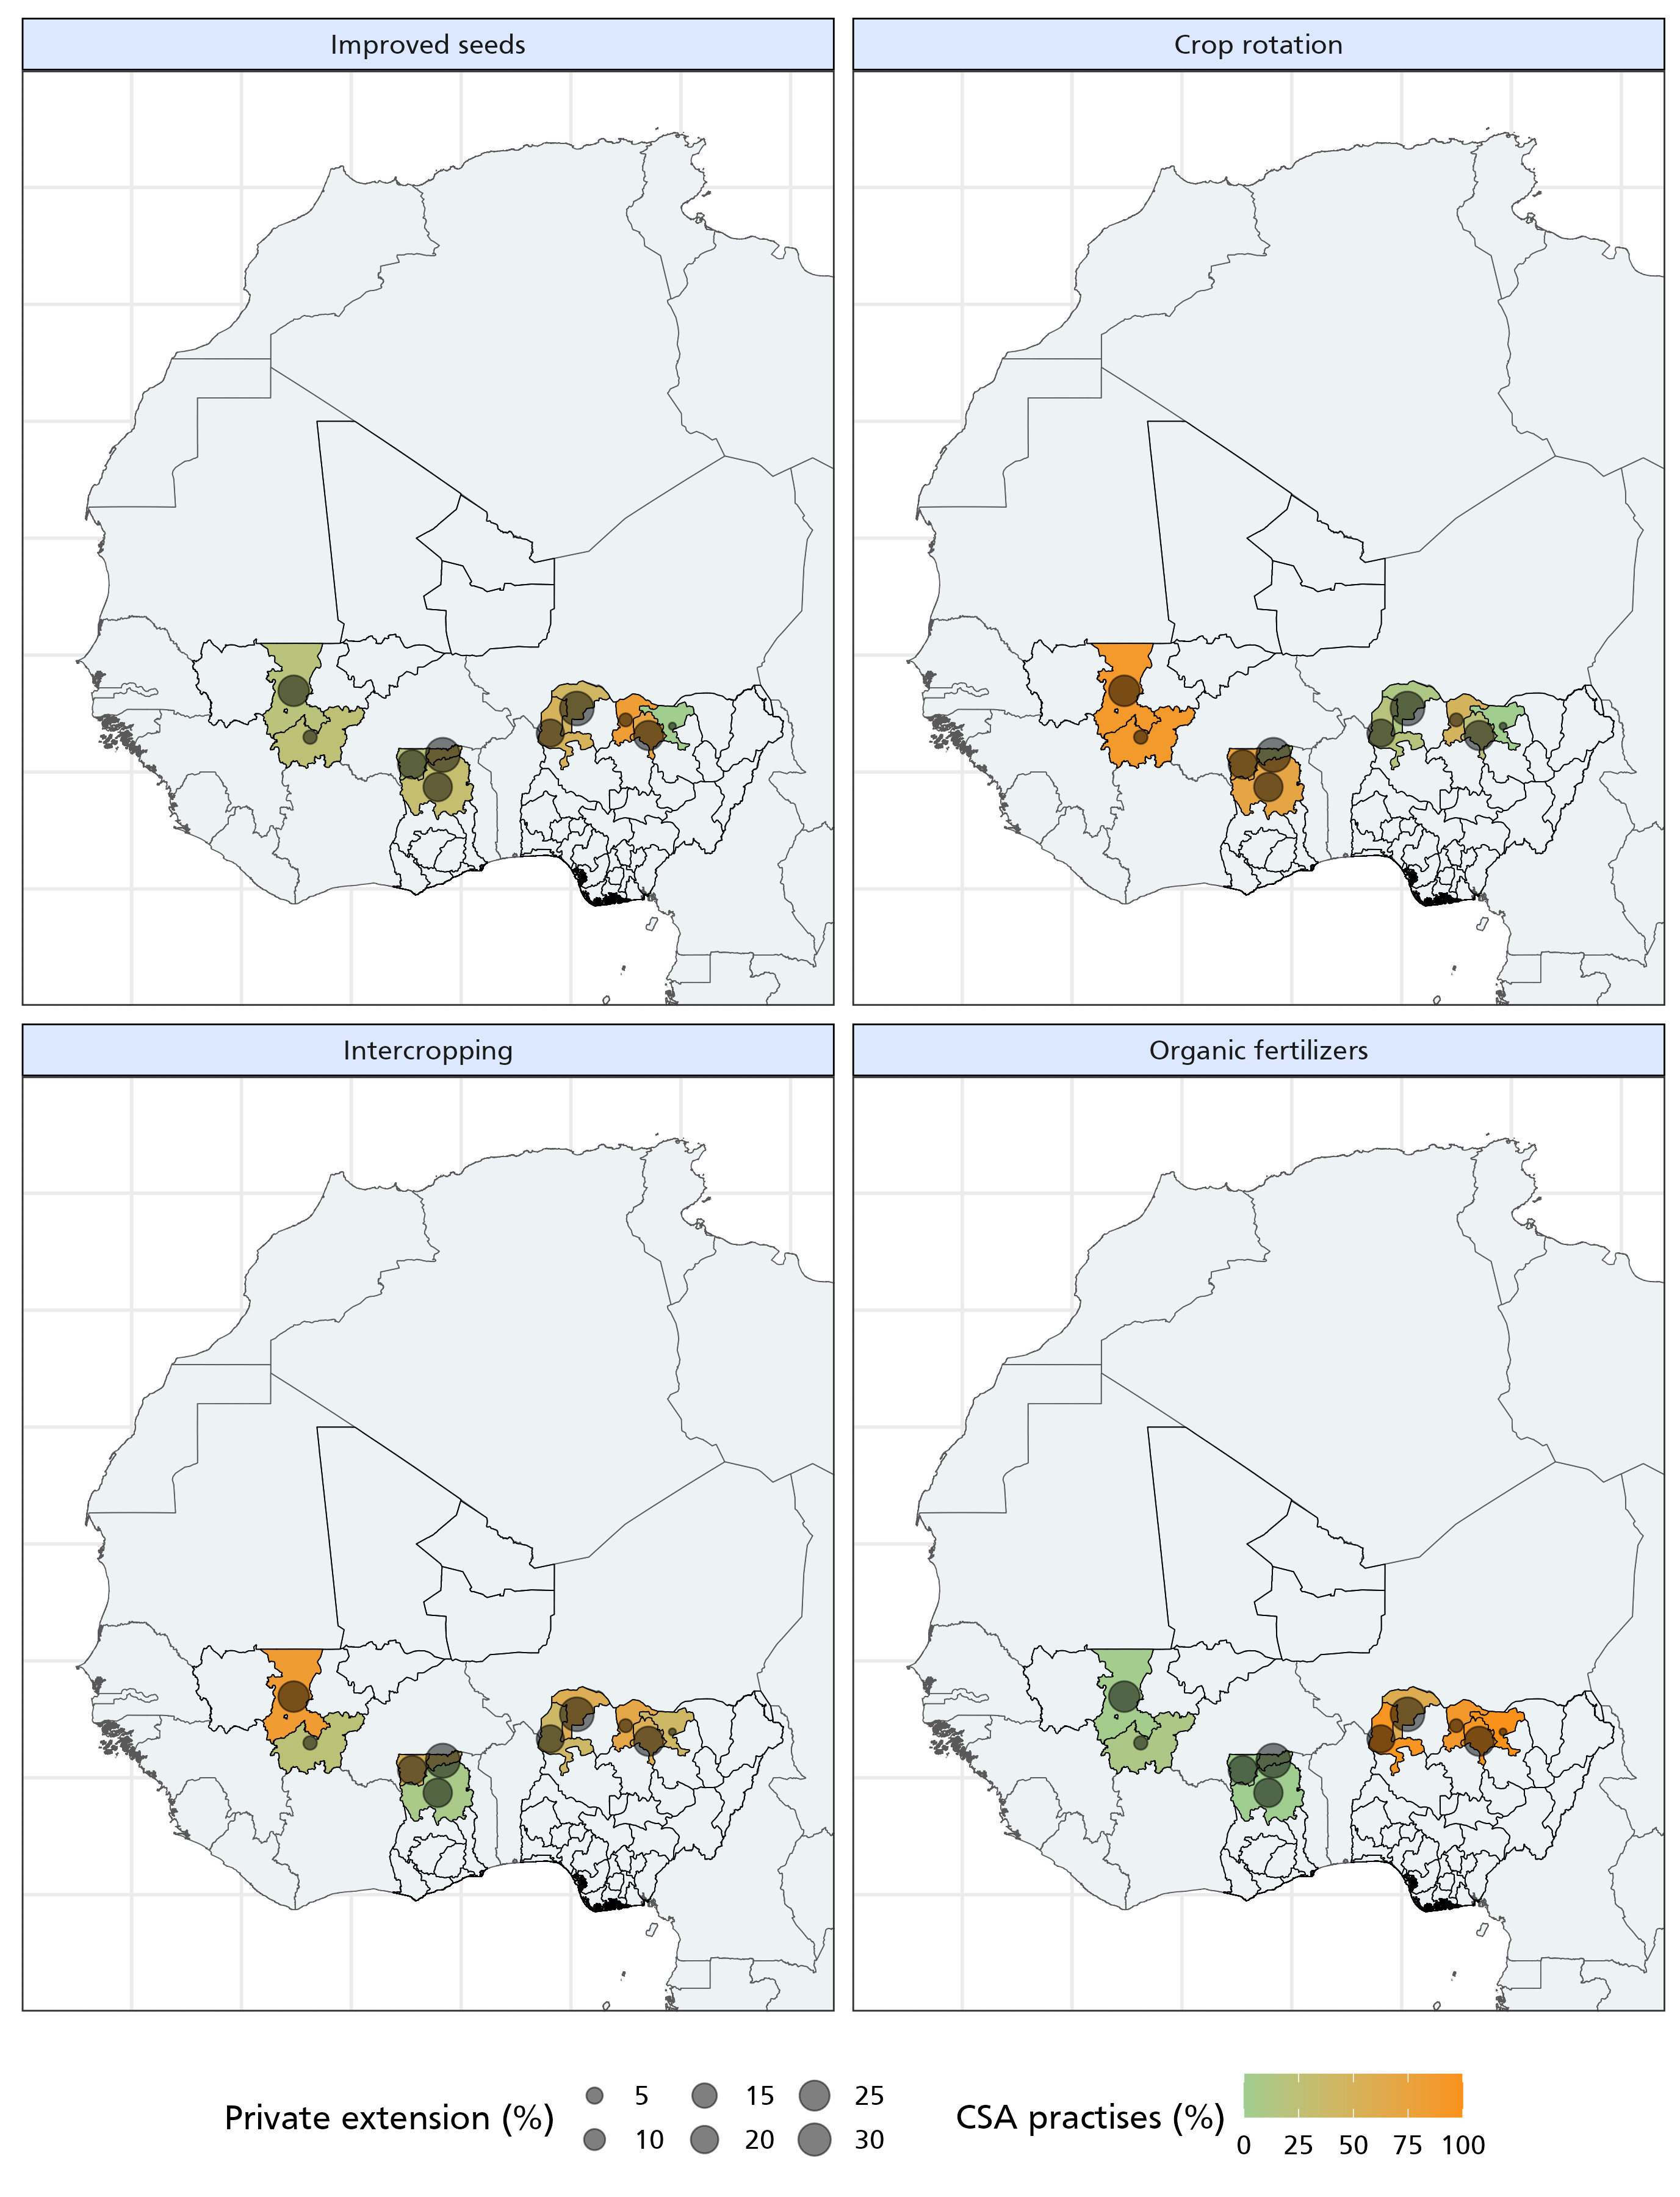
\includegraphics[scale=0.6]{"figures/map_private.png"}
\caption{Private extension system and CSA practises  by region (2019)}
\caption*{Note: The map illustrates the CSA practices in Ghana, Mali and Nigeria. The shaded areas on the map indicate the percentage of households adopting these CSA practices, with varying intensities of shade representing different levels of adoption: the lightest shade denotes 0-25\% adoption, followed by a light shade for 26-50\%, a medium shade for 51-75\%, and a dark shade for 76-100\% of adoption. Overlaid on these shaded regions are points of varying sizes, each representing the extent of access to private extension services in different regions of the country. The size of these points corresponds to the percentage of households with access to these services: the smallest points indicate 0-5\% access, increasing in size from 6-10\%, 11-15\%, 16-20\%, 21 -25\% , 25-30\% and the largest points for more than 30\% access.}
\label{fig:map_1}
\end{figure}

\newpage
\begin{figure}[H]
\centering
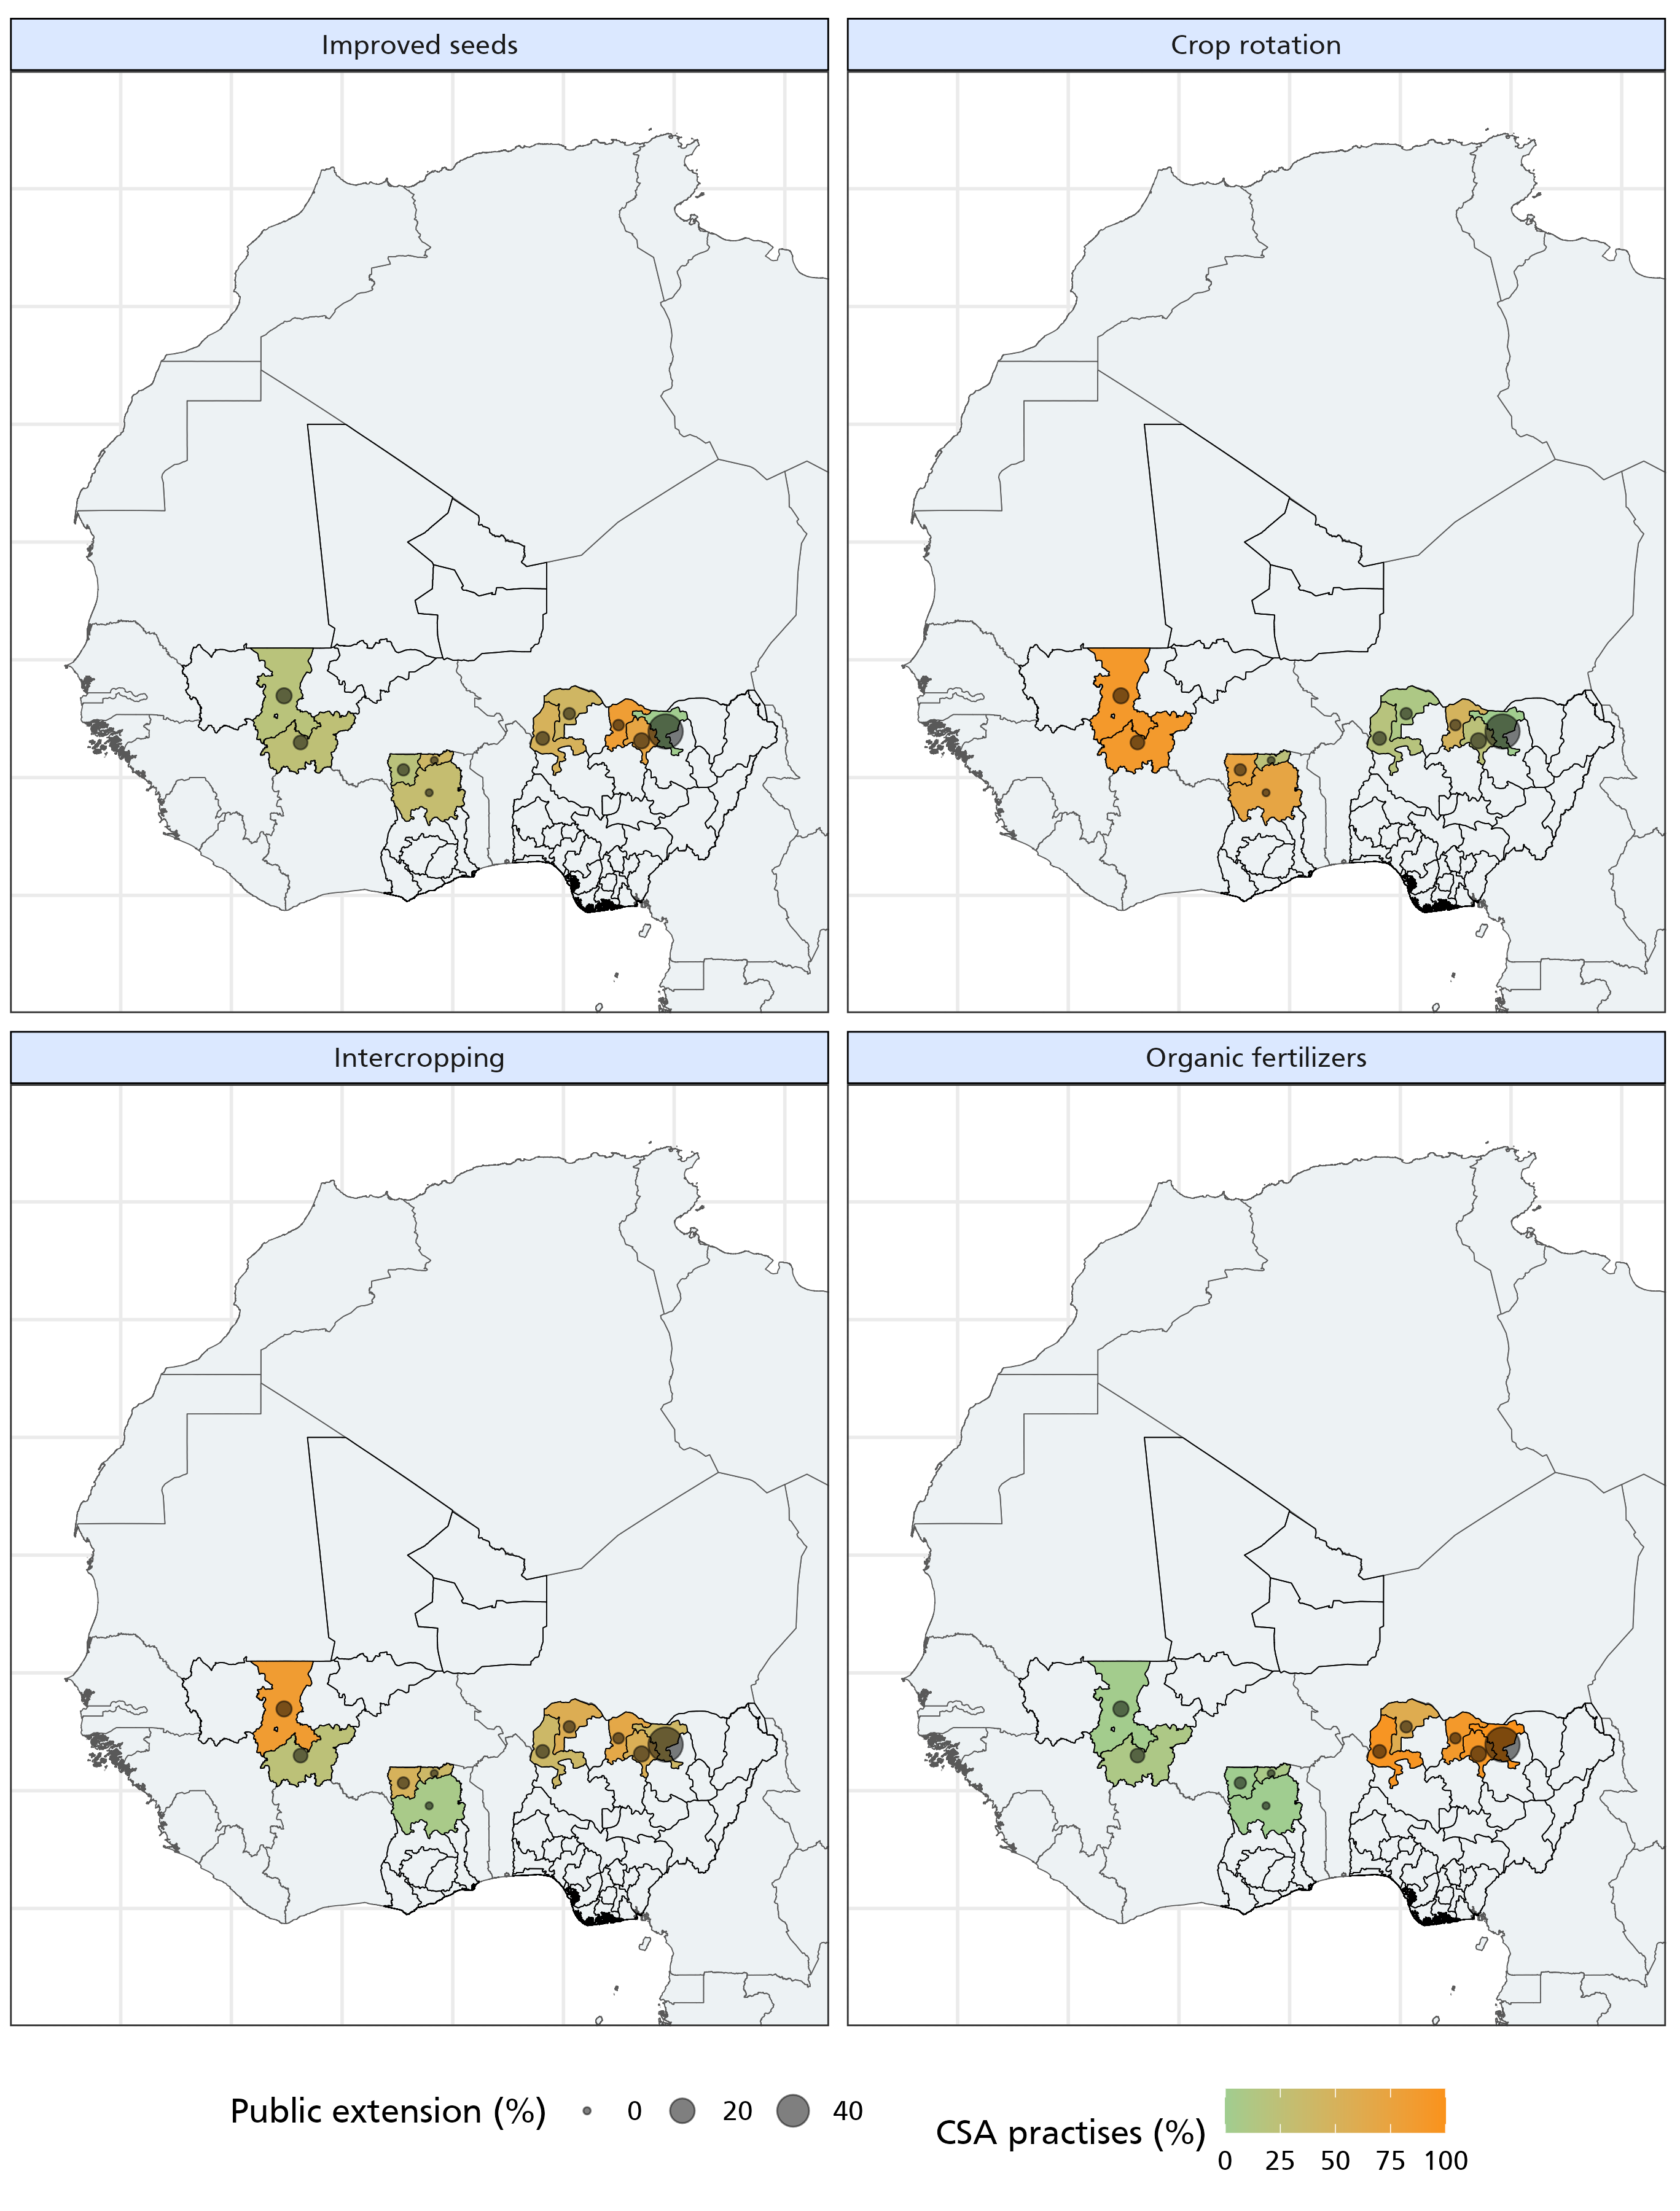
\includegraphics[scale=0.6]{"figures/map_public.png"}
\caption{Public extension system and CSA practises  by region (2019)}
\caption*{Note: The map illustrates the CSA practices in Ghana, Mali and Nigeria. The shaded areas on the map indicate the percentage of households adopting these CSA practices, with varying intensities of shade representing different levels of adoption: the lightest shade denotes 0-25\% adoption, followed by a light shade for 26-50\%, a medium shade for 51-75\%, and a dark shade for 76-100\% of adoption. Overlaid on these shaded regions are points of varying sizes, each representing the extent of access to public extension services in different regions of the country. The size of these points corresponds to the percentage of households with access to these services: the smallest points indicate 0\% access, increasing to 0-20\%, 20-40\%, and the largest points for more than 40\% access.}
\label{fig:map_1}
\end{figure}

\begin{figure}[H]
\centering
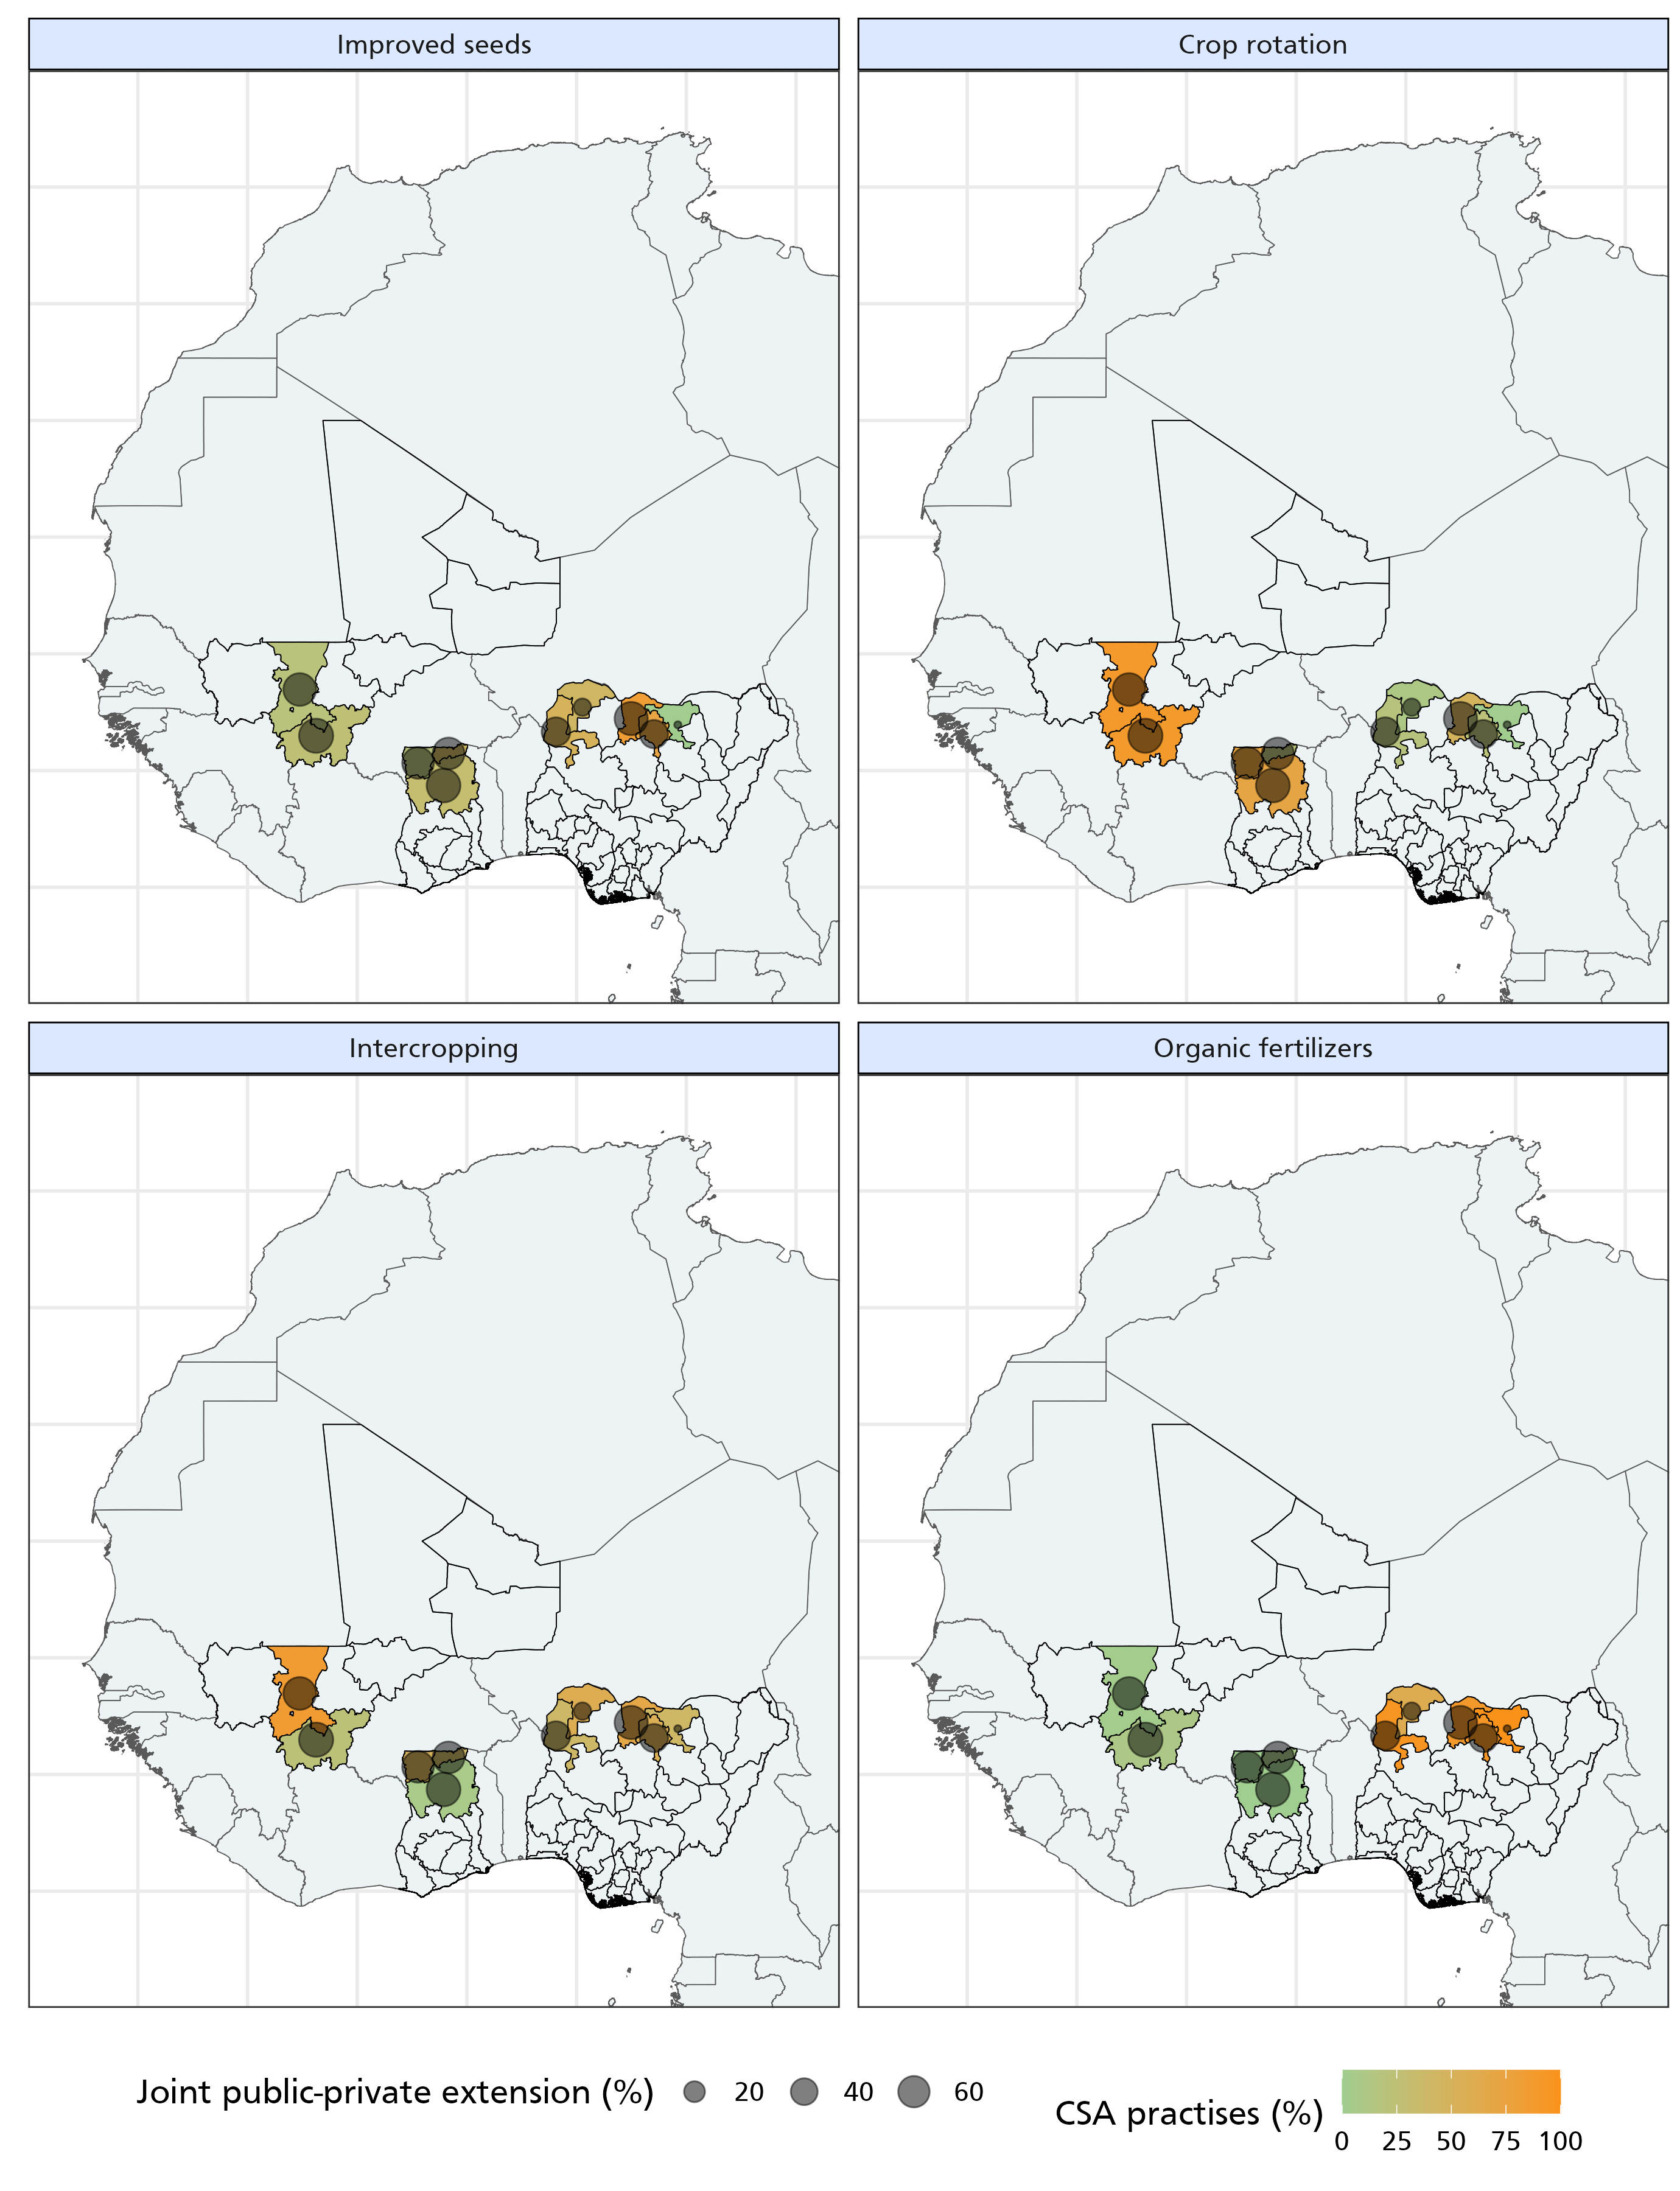
\includegraphics[scale=0.6]{"figures/map_joint.png"}
\caption{Note: Joint Public-private extension system and CSA practises  by region (2019)}
\caption*{The map illustrates the CSA practices in Ghana, Mali and Nigeria. The shaded areas on the map indicate the percentage of households adopting these CSA practices, with varying intensities of shade representing different levels of adoption: the lightest shade denotes 0-25\% adoption, followed by a light shade for 26-50\%, a medium shade for 51-75\%, and a dark shade for 76-100\% of adoption. Overlaid on these shaded regions are points of varying sizes, each representing the extent of access to joint public-private extension services in different regions of the country. The size of these points corresponds to the percentage of households with access to these services: the smallest points indicate 0\% access, increasing to 0-20\%, 20-40\%,40-60\% and the largest points for more than 60\% access.}
\label{fig:map_1}
\end{figure}

\clearpage

\begingroup\fontsize{7}{9}\selectfont

\begin{longtable}[t]{lrrrr}
\caption{\label{tab:unnamed-chunk-3}Access to extension services and CSA - (CRE) (Without Controls)}\\
\toprule
Variables & Crop rotation & Improved seeds & Intercropping & Organic fertilisers\\
\midrule
\endfirsthead
\caption[]{\label{tab:unnamed-chunk-3}Access to extension services and CSA - (CRE) (Without Controls) \textit{(continued)}}\\
\toprule
Variables & Crop rotation & Improved seeds & Intercropping & Organic fertilisers\\
\midrule
\endhead

\endfoot
\bottomrule
\endlastfoot
Private extension & 0.185 & \textbf{-0.552**} & -0.290 & \textbf{-0.883***}\\
 & (0.397) & (0.240) & (0.231) & (0.224)\\
Public extension & \textbf{0.527***} & -0.0885 & 0.175 & \textbf{-0.606***}\\
 & (0.201) & (0.208) & (0.144) & (0.194)\\
Joint Public-private extension & \textbf{0.607***} & \textbf{0.524**} & 0.00917 & \textbf{-0.376*}\\
 & (0.183) & (0.238) & (0.171) & (0.219)\\
Constant & \textbf{-0.482**} & \textbf{-0.502**} & \textbf{-0.313***} & 0.252\\
 & (0.191) & (0.244) & (0.118) & (0.188)\\
\midrule
Observations & 8,604 & 8,604 & 8,604 & 8,604\\
Additional controls & No & No & No & No\\
District FE & No & No & No & No\\
Year FE & Yes & Yes & Yes & Yes\\
\midrule
Robust standard errors in parentheses &  &  &  & \\
*** p<0.01, ** p<0.05, * p<0.1 &  &  &  & \\*
\end{longtable}
\endgroup{}

\newpage

\begingroup\fontsize{7}{9}\selectfont

\begin{longtable}[t]{lrrrr}
\caption{\label{tab:unnamed-chunk-4}Access to extension services and CSA - (CRE)}\\
\toprule
Variables & Crop rotation & Improved seeds & Intercropping & Organic fertilisers\\
\midrule
\endfirsthead
\caption[]{\label{tab:unnamed-chunk-4}Access to extension services and CSA - (CRE) \textit{(continued)}}\\
\toprule
Variables & Crop rotation & Improved seeds & Intercropping & Organic fertilisers\\
\midrule
\endhead

\endfoot
\bottomrule
\endlastfoot
Private extension & -0.0118 & 0.277 & \textbf{0.343***} & -0.149\\
 & (0.195) & (0.231) & (0.133) & (0.391)\\
Public extension & \textbf{0.178*} & 0.0161 & \textbf{0.378**} & 0.00671\\
 & (0.104) & (0.161) & (0.150) & (0.129)\\
Joint Public-private extension & \textbf{0.284**} & \textbf{0.842***} & 0.253 & 0.295\\
 & (0.127) & (0.222) & (0.154) & (0.191)\\
Age of household head (years) & 0.0139 & -0.00917 & 0.0625 & -0.0953\\
 & (0.0812) & (0.0957) & (0.0809) & (0.0919)\\
Sex of household head (dummy, male=1) & 0.133 & \textbf{0.209*} & -0.0630 & -0.0245\\
 & (0.119) & (0.111) & (0.111) & (0.247)\\
Education level (Number of years) & -0.00311 & \textbf{0.0112*} & -0.00896 & -0.00210\\
 & (0.00905) & (0.00676) & (0.0106) & (0.00617)\\
Household size (number of persons) & 0.00605 & -0.0113 & \textbf{0.0214***} & \textbf{-0.0240**}\\
 & (0.00649) & (0.0102) & (0.00674) & (0.0107)\\
Distance to the nearest urban market (km) & \textbf{0.00943**} & -0.00599 & 0.000657 & 0.00240\\
 & (0.00419) & (0.00730) & (0.00533) & (0.00614)\\
Distance the nearest village market (km) & \textbf{-0.0206**} & 0.00989 & \textbf{-0.0219**} & -0.0263\\
 & (0.00896) & (0.00997) & (0.0107) & (0.0166)\\
Cooperative membership (dummy) & 0.0819 & -0.00866 & -0.0605 & 0.130\\
 & (0.108) & (0.0783) & (0.132) & (0.114)\\
Labor cost (USD/ha) & 0.000652 & \textbf{0.00373***} & 0.000473 & \textbf{0.00685***}\\
 & (0.00160) & (0.00139) & (0.00136) & (0.00207)\\
Groundnut area (ha) & \textbf{0.158***} & 0.0378 & \textbf{0.0684*} & \textbf{0.228***}\\
 & (0.0506) & (0.0326) & (0.0379) & (0.0848)\\
Off-farm income (dummy) & 0.00842 & 0.220 & 0.0102 & -0.341\\
 & (0.154) & (0.225) & (0.154) & (0.256)\\
Dependency ratio & -0.00586 & -0.0215 & \textbf{0.0515**} & \textbf{0.0832**}\\
 & (0.0227) & (0.0318) & (0.0236) & (0.0353)\\
Clay soil (dummy) & \textbf{0.136***} & -0.00972 & 0.0280 & 0.0604\\
 & (0.0526) & (0.0526) & (0.0533) & (0.0854)\\
Sandy-clay soil (dummy) & \textbf{0.113*} & 0.000136 & 0.0290 & \textbf{0.119**}\\
 & (0.0593) & (0.0561) & (0.0396) & (0.0570)\\
Silty soil (dummy) & \textbf{0.169**} & -0.00204 & -0.0224 & 0.0321\\
 & (0.0666) & (0.0673) & (0.0509) & (0.0817)\\
agebar & -0.0164 & 0.00874 & -0.0603 & 0.0964\\
 & (0.0811) & (0.0951) & (0.0806) & (0.0916)\\
hhsizebar & -0.00718 & 0.0137 & \textbf{-0.0255***} & 0.0103\\
 & (0.00980) & (0.0120) & (0.00834) & (0.0115)\\
gsizebar & -0.0476 & \textbf{0.0904***} & -0.0266 & -0.0915\\
 & (0.0479) & (0.0324) & (0.0352) & (0.0739)\\
off\_farmbar & 0.0512 & -0.166 & 0.0508 & 0.272\\
 & (0.178) & (0.163) & (0.155) & (0.281)\\
dratiobar & 0.00862 & 0.0313 & -0.0458 & -0.0435\\
 & (0.0250) & (0.0365) & (0.0286) & (0.0394)\\
Constant & \textbf{-1.845***} & \textbf{-0.500*} & -0.290 & \textbf{-1.264***}\\
\midrule
 & (0.188) & (0.272) & (0.259) & (0.436)\\
Observations & 8,604 & 8,604 & 8,604 & 8,604\\
Additional controls & Yes & Yes & Yes & Yes\\
District FE & Yes & Yes & Yes & Yes\\
Year FE & Yes & Yes & Yes & Yes\\
\midrule
Robust standard errors in parentheses &  &  &  & \\
*** p<0.01, ** p<0.05, * p<0.1 &  &  &  & \\*
\end{longtable}
\endgroup{}

\newpage

\begingroup\fontsize{7}{9}\selectfont

\begin{longtable}[t]{lrrrr}
\caption{\label{tab:unnamed-chunk-5}Access to extension services and CSA - (CRE) (Ghana)}\\
\toprule
Variables & Crop rotation & Improved seeds & Intercropping & Organic fertilisers\\
\midrule
\endfirsthead
\caption[]{\label{tab:unnamed-chunk-5}Access to extension services and CSA - (CRE) (Ghana) \textit{(continued)}}\\
\toprule
Variables & Crop rotation & Improved seeds & Intercropping & Organic fertilisers\\
\midrule
\endhead

\endfoot
\bottomrule
\endlastfoot
Private extension & \textbf{-0.909*} & 0 & \textbf{-1.042**} & \textbf{0.936***}\\
 & (0.540) & 0 & (0.447) & (0.100)\\
Public extension & -0.134 & \textbf{1.180***} & -0.0590 & 0.0992\\
 & (0.175) & (0.425) & (0.226) & (0.266)\\
Joint Public-private extension & 0.0418 & \textbf{2.336***} & -0.0913 & 0\\
 & (0.148) & (0.379) & (0.263) & 0\\
Age of household head (years) & -0.267 & -0.202 & 0.103 & -0.107\\
 & (0.172) & (0.165) & (0.197) & (0.180)\\
Sex of household head (dummy, male=1) & 0.0430 & 0.166 & \textbf{-0.314**} & 0.332\\
 & (0.146) & (0.191) & (0.149) & (0.258)\\
Education level (Number of years) & -0.0103 & \textbf{0.0337**} & \textbf{0.0192*} & -0.0196\\
 & (0.0185) & (0.0143) & (0.0115) & (0.0141)\\
Household size (number of persons) & -0.0200 & 0.0176 & -0.0303 & \textbf{0.0701***}\\
 & (0.0345) & (0.0179) & (0.0198) & (0.0199)\\
Distance to the nearest urban market (km) & -0.0319 & 0.00251 & 0.0254 & \textbf{0.180***}\\
 & (0.0259) & (0.0153) & (0.0205) & (0.0551)\\
Distance the nearest village market (km) & -0.0168 & -0.0197 & -0.0393 & \textbf{-0.113***}\\
 & (0.0204) & (0.0248) & (0.0330) & (0.0417)\\
Cooperative membership (dummy) & \textbf{0.518***} & 0.241 & 0.0564 & 0.454\\
 & (0.193) & (0.184) & (0.208) & (0.301)\\
Labor cost (USD/ha) & 0.00312 & \textbf{0.0111***} & 0.000712 & 0.00175\\
 & (0.00226) & (0.00228) & (0.00199) & (0.00125)\\
Groundnut area (ha) & \textbf{0.333**} & 0.0419 & -0.0511 & \textbf{0.528***}\\
 & (0.139) & (0.0675) & (0.105) & (0.0859)\\
Off-farm income (dummy) & 0.519 & -0.431 & \textbf{0.712***} & \textbf{1.961***}\\
 & (0.733) & (0.334) & (0.169) & (0.282)\\
Dependency ratio & \textbf{0.0903*} & -0.00890 & 0.0111 & 0.0252\\
 & (0.0547) & (0.0514) & (0.0890) & (0.116)\\
Clay soil (dummy) & \textbf{0.245**} & -0.00160 & -0.0609 & \textbf{0.532***}\\
 & (0.105) & (0.0822) & (0.118) & (0.161)\\
Sandy-clay soil (dummy) & \textbf{0.224***} & 0.133 & -0.0752 & \textbf{0.613***}\\
 & (0.0869) & (0.0908) & (0.116) & (0.213)\\
Silty soil (dummy) & \textbf{0.365**} & 0.106 & -0.182 & 0.243\\
 & (0.184) & (0.0907) & (0.206) & (0.156)\\
agebar & 0.255 & 0.195 & -0.0964 & 0.0791\\
 & (0.171) & (0.163) & (0.197) & (0.183)\\
hhsizebar & 0.0325 & 0.00467 & 0.0166 & \textbf{0.0692**}\\
 & (0.0475) & (0.0259) & (0.0164) & (0.0281)\\
gsizebar & -0.0298 & 0.0171 & -0.0412 & 0.239\\
 & (0.0881) & (0.0721) & (0.123) & (0.162)\\
off\_farmbar & -0.154 & 0.564 & -0.345 & \textbf{-2.104***}\\
 & (0.612) & (0.389) & (0.448) & (0.449)\\
dratiobar & -0.0672 & -0.0701 & -0.0718 & 0.0361\\
 & (0.0700) & (0.0903) & (0.0825) & (0.163)\\
Constant & 0.390 & \textbf{-1.844***} & -0.547 & \textbf{-6.351***}\\
\midrule
 & (0.504) & (0.426) & (0.347) & (1.081)\\
Observations & 1,494 & 1,494 & 1,494 & 1,494\\
Additional controls & Yes & Yes & Yes & Yes\\
District FE & Yes & Yes & Yes & Yes\\
Year FE & Yes & Yes & Yes & Yes\\
\midrule
Robust standard errors in parentheses &  &  &  & \\
*** p<0.01, ** p<0.05, * p<0.1 &  &  &  & \\*
\end{longtable}
\endgroup{}

\newpage

\begingroup\fontsize{7}{9}\selectfont

\begin{longtable}[t]{lrrrr}
\caption{\label{tab:unnamed-chunk-6}Access to extension services and CSA - (CRE) (Mali)}\\
\toprule
Variables & Crop rotation & Improved seeds & Intercropping & Organic fertilisers\\
\midrule
\endfirsthead
\caption[]{\label{tab:unnamed-chunk-6}Access to extension services and CSA - (CRE) (Mali) \textit{(continued)}}\\
\toprule
Variables & Crop rotation & Improved seeds & Intercropping & Organic fertilisers\\
\midrule
\endhead

\endfoot
\bottomrule
\endlastfoot
Private extension & 0.0116 & 0.0223 & \textbf{0.385***} & -0.0803\\
 & (0.299) & (0.274) & (0.122) & (0.115)\\
Public extension & \textbf{0.580***} & 0.159 & 0.356 & \textbf{-0.689***}\\
 & (0.167) & (0.394) & (0.264) & (0.170)\\
Joint Public-private extension & 0.192 & \textbf{1.610***} & \textbf{0.408*} & \textbf{0.312**}\\
 & (0.255) & (0.335) & (0.240) & (0.133)\\
Age of household head (years) & 0.134 & \textbf{-0.164**} & 0.0618 & -0.126\\
 & (0.119) & (0.0664) & (0.133) & (0.124)\\
Sex of household head (dummy, male=1) & 0.117 & 0.157 & 0.179 & -0.305\\
 & (0.223) & (0.212) & (0.128) & (0.192)\\
Education level (Number of years) & \textbf{0.0596***} & \textbf{0.0656***} & \textbf{-0.0487***} & -0.0127\\
 & (0.0173) & (0.0150) & (0.0158) & (0.0241)\\
Household size (number of persons) & \textbf{0.0116**} & -0.00707 & \textbf{0.0263***} & -0.00501\\
 & (0.00521) & (0.00722) & (0.00713) & (0.0137)\\
Distance to the nearest urban market (km) & \textbf{0.00990**} & 0.00278 & 0.00178 & \textbf{-0.00661***}\\
 & (0.00473) & (0.00771) & (0.0147) & (0.00188)\\
Distance the nearest village market (km) & -0.0178 & 0.0151 & \textbf{-0.0234**} & -0.0230\\
 & (0.0119) & (0.0121) & (0.0112) & (0.0176)\\
Cooperative membership (dummy) & -0.0768 & -0.0613 & \textbf{-0.441***} & 0.113\\
 & (0.183) & (0.104) & (0.136) & (0.143)\\
Labor cost (USD/ha) & 0.00196 & 0.00224 & -0.00125 & -0.00349\\
 & (0.00357) & (0.00238) & (0.00301) & (0.00272)\\
Groundnut area (ha) & \textbf{0.127***} & 0.0146 & 0.00203 & 0.00461\\
 & (0.0440) & (0.0142) & (0.0280) & (0.0605)\\
Off-farm income (dummy) & 0.191 & \textbf{-0.363*} & \textbf{1.044***} & \textbf{0.797*}\\
 & (0.432) & (0.212) & (0.324) & (0.436)\\
Dependency ratio & -0.00222 & -0.0334 & 0.0436 & 0.0316\\
 & (0.0909) & (0.0403) & (0.0581) & (0.0467)\\
Clay soil (dummy) & 0.0780 & -0.0710 & 0.0548 & -0.188\\
 & (0.115) & (0.105) & (0.123) & (0.118)\\
Sandy-clay soil (dummy) & -0.0568 & -0.0963 & -0.0104 & 0.0110\\
 & (0.132) & (0.0760) & (0.0937) & (0.128)\\
Silty soil (dummy) & \textbf{0.234**} & -0.141 & -0.0434 & -0.0106\\
 & (0.111) & (0.158) & (0.0848) & (0.182)\\
agebar & -0.141 & \textbf{0.168**} & -0.0584 & 0.125\\
 & (0.117) & (0.0681) & (0.134) & (0.124)\\
hhsizebar & \textbf{-0.0165*} & 0.0162 & \textbf{-0.0316***} & -0.00359\\
 & (0.00954) & (0.00992) & (0.00801) & (0.0157)\\
gsizebar & 0.0215 & \textbf{0.0866**} & -0.0406 & 0.00398\\
 & (0.0341) & (0.0361) & (0.0388) & (0.0871)\\
off\_farmbar & -0.424 & -0.0412 & -0.378 & -0.0192\\
 & (0.628) & (0.322) & (0.885) & (0.641)\\
dratiobar & 0.0138 & -0.0309 & -0.0735 & 0.0217\\
 & (0.0561) & (0.0707) & (0.0856) & (0.0898)\\
Constant & \textbf{1.690***} & \textbf{-2.743***} & -0.464 & \textbf{-0.619**}\\
\midrule
 & (0.369) & (0.565) & (0.434) & (0.269)\\
Observations & 2,520 & 2,520 & 2,520 & 2,520\\
Additional controls & Yes & Yes & Yes & Yes\\
District FE & Yes & Yes & Yes & Yes\\
Year FE & Yes & Yes & Yes & Yes\\
\midrule
Robust standard errors in parentheses &  &  &  & \\
*** p<0.01, ** p<0.05, * p<0.1 &  &  &  & \\*
\end{longtable}
\endgroup{}

\newpage

\begingroup\fontsize{7}{9}\selectfont

\begin{longtable}[t]{lrrrr}
\caption{\label{tab:unnamed-chunk-7}Access to extension services and CSA - (CRE) (Nigeria)}\\
\toprule
Variables & Crop rotation & Improved seeds & Intercropping & Organic fertilisers\\
\midrule
\endfirsthead
\caption[]{\label{tab:unnamed-chunk-7}Access to extension services and CSA - (CRE) (Nigeria) \textit{(continued)}}\\
\toprule
Variables & Crop rotation & Improved seeds & Intercropping & Organic fertilisers\\
\midrule
\endhead

\endfoot
\bottomrule
\endlastfoot
Private extension & 0.152 & \textbf{0.717***} & \textbf{0.519*} & -0.207\\
 & (0.312) & (0.265) & (0.273) & (0.425)\\
Public extension & 0.0638 & 0.0660 & \textbf{0.471*} & 0.218\\
 & (0.146) & (0.172) & (0.242) & (0.166)\\
Joint Public-private extension & \textbf{0.455***} & \textbf{0.471*} & 0.184 & 0.0353\\
 & (0.152) & (0.242) & (0.174) & (0.246)\\
Age of household head (years) & 0.0698 & 0.0664 & 0.0664 & -0.000880\\
 & (0.0966) & (0.142) & (0.113) & (0.110)\\
Sex of household head (dummy, male=1) & \textbf{0.420*} & -0.0769 & 0.207 & 0.111\\
 & (0.230) & (0.133) & (0.242) & (0.267)\\
Education level (Number of years) & -0.0110 & -0.00321 & -0.0126 & -0.00915\\
 & (0.0126) & (0.00649) & (0.0137) & (0.00637)\\
Household size (number of persons) & -0.00181 & -0.0142 & 0.0178 & \textbf{-0.0454**}\\
 & (0.0114) & (0.0195) & (0.0126) & (0.0208)\\
Distance to the nearest urban market (km) & \textbf{0.0108**} & -0.00853 & -0.00109 & 0.00379\\
 & (0.00469) & (0.00985) & (0.00487) & (0.00756)\\
Distance the nearest village market (km) & \textbf{-0.0494*} & 0.0270 & -0.00474 & -0.00224\\
 & (0.0277) & (0.0303) & (0.0338) & (0.0306)\\
Cooperative membership (dummy) & -0.0130 & 0.0321 & 0.149 & 0.103\\
 & (0.105) & (0.0821) & (0.243) & (0.140)\\
Labor cost (USD/ha) & -0.000566 & 0.00300 & 0.00110 & \textbf{0.0171***}\\
 & (0.00187) & (0.00186) & (0.00181) & (0.00440)\\
Groundnut area (ha) & 0.0800 & 0.0742 & \textbf{0.176***} & \textbf{0.551***}\\
 & (0.0489) & (0.0629) & (0.0605) & (0.126)\\
Off-farm income (dummy) & -0.0387 & 0.176 & -0.109 & \textbf{-0.487*}\\
 & (0.127) & (0.221) & (0.161) & (0.284)\\
Dependency ratio & -0.0182 & -0.0155 & \textbf{0.0715**} & 0.0757\\
 & (0.0223) & (0.0425) & (0.0279) & (0.0473)\\
Clay soil (dummy) & 0.122 & 0.0296 & 0.0820 & 0.147\\
 & (0.0770) & (0.0812) & (0.0634) & (0.0937)\\
Sandy-clay soil (dummy) & \textbf{0.164***} & 0.0253 & \textbf{0.0884**} & \textbf{0.133**}\\
 & (0.0612) & (0.0834) & (0.0352) & (0.0533)\\
Silty soil (dummy) & 0.0534 & 0.0490 & 0.0414 & -0.00442\\
 & (0.0889) & (0.0874) & (0.0514) & (0.0735)\\
agebar & -0.0648 & -0.0649 & -0.0681 & 0.00229\\
 & (0.0964) & (0.141) & (0.112) & (0.110)\\
hhsizebar & -0.00656 & -0.00412 & -0.0129 & 0.0321\\
 & (0.0209) & (0.0246) & (0.0168) & (0.0257)\\
gsizebar & -0.0295 & \textbf{0.101*} & 0.0115 & \textbf{-0.157*}\\
 & (0.0601) & (0.0613) & (0.0498) & (0.0931)\\
off\_farmbar & 0.125 & -0.124 & 0.101 & 0.272\\
 & (0.163) & (0.168) & (0.168) & (0.283)\\
dratiobar & 0.0206 & 0.0547 & -0.0483 & -0.0355\\
 & (0.0334) & (0.0467) & (0.0294) & (0.0380)\\
Constant & \textbf{-2.022***} & -0.128 & \textbf{-1.063**} & 0.387\\
\midrule
 & (0.364) & (0.409) & (0.486) & (0.370)\\
Observations & 4,590 & 4,590 & 4,590 & 4,590\\
Additional controls & Yes & Yes & Yes & Yes\\
District FE & Yes & Yes & Yes & Yes\\
Year FE & Yes & Yes & Yes & Yes\\
\midrule
Robust standard errors in parentheses &  &  &  & \\
*** p<0.01, ** p<0.05, * p<0.1 &  &  &  & \\*
\end{longtable}
\endgroup{}

\newpage

\begin{table}[htbp]
\caption{Coefficient stability and Unobserved selection}
\begin{tabular}{@{}llrrr@{}}
\toprule
                   &              & Private extension & Public extension & Joint Public-Private extension \\ \midrule
Croprotation       & Beta         & 0.059          & 0.026            & 0.13                           \\
                   & Delta        & -2.69             & -1.17            & 5.88                           \\
                   & $R^2_{max}$      & 0.078             & 0.078            & 0.078                          \\
                   & Observations & 8604              & 8604             & 8604                           \\ \midrule
Improved seed      & Beta         & 0.11              & 0.086            & 0.18                           \\
                   & Delta        & -2.66             & -0.51            & 1.95                           \\
                   & $R^2_{max}$      & 0.075             & 0.075            & 0.075                          \\
                   & Observations & 8604              & 8604             & 8604                           \\ \midrule
Intercropping      & Beta         & 0.2               & 0.22             & 0.2                            \\
                   & Delta        & -5.41             & -5.62            & -95.53                         \\
                   & $R^2_{max}$      & 0.073             & 0.073            & 0.073                          \\
                   & Observations & 8604              & 8604             & 8604                           \\ \midrule
Organic fertilizer & Beta         & -0.027            & -0.012           & 0.012                          \\
                   & Delta        & 2.35              & 3.65             & 1.39                           \\
                   & $R^2_{max}$      & 0.11              & 0.11             & 0.11                           \\
                   & Observations & 8604              & 8604             & 8604                           \\ \bottomrule
\end{tabular}
\end{table}

\pagebreak
\newpage

\newpage

\begin{figure}[htbp]
\centering
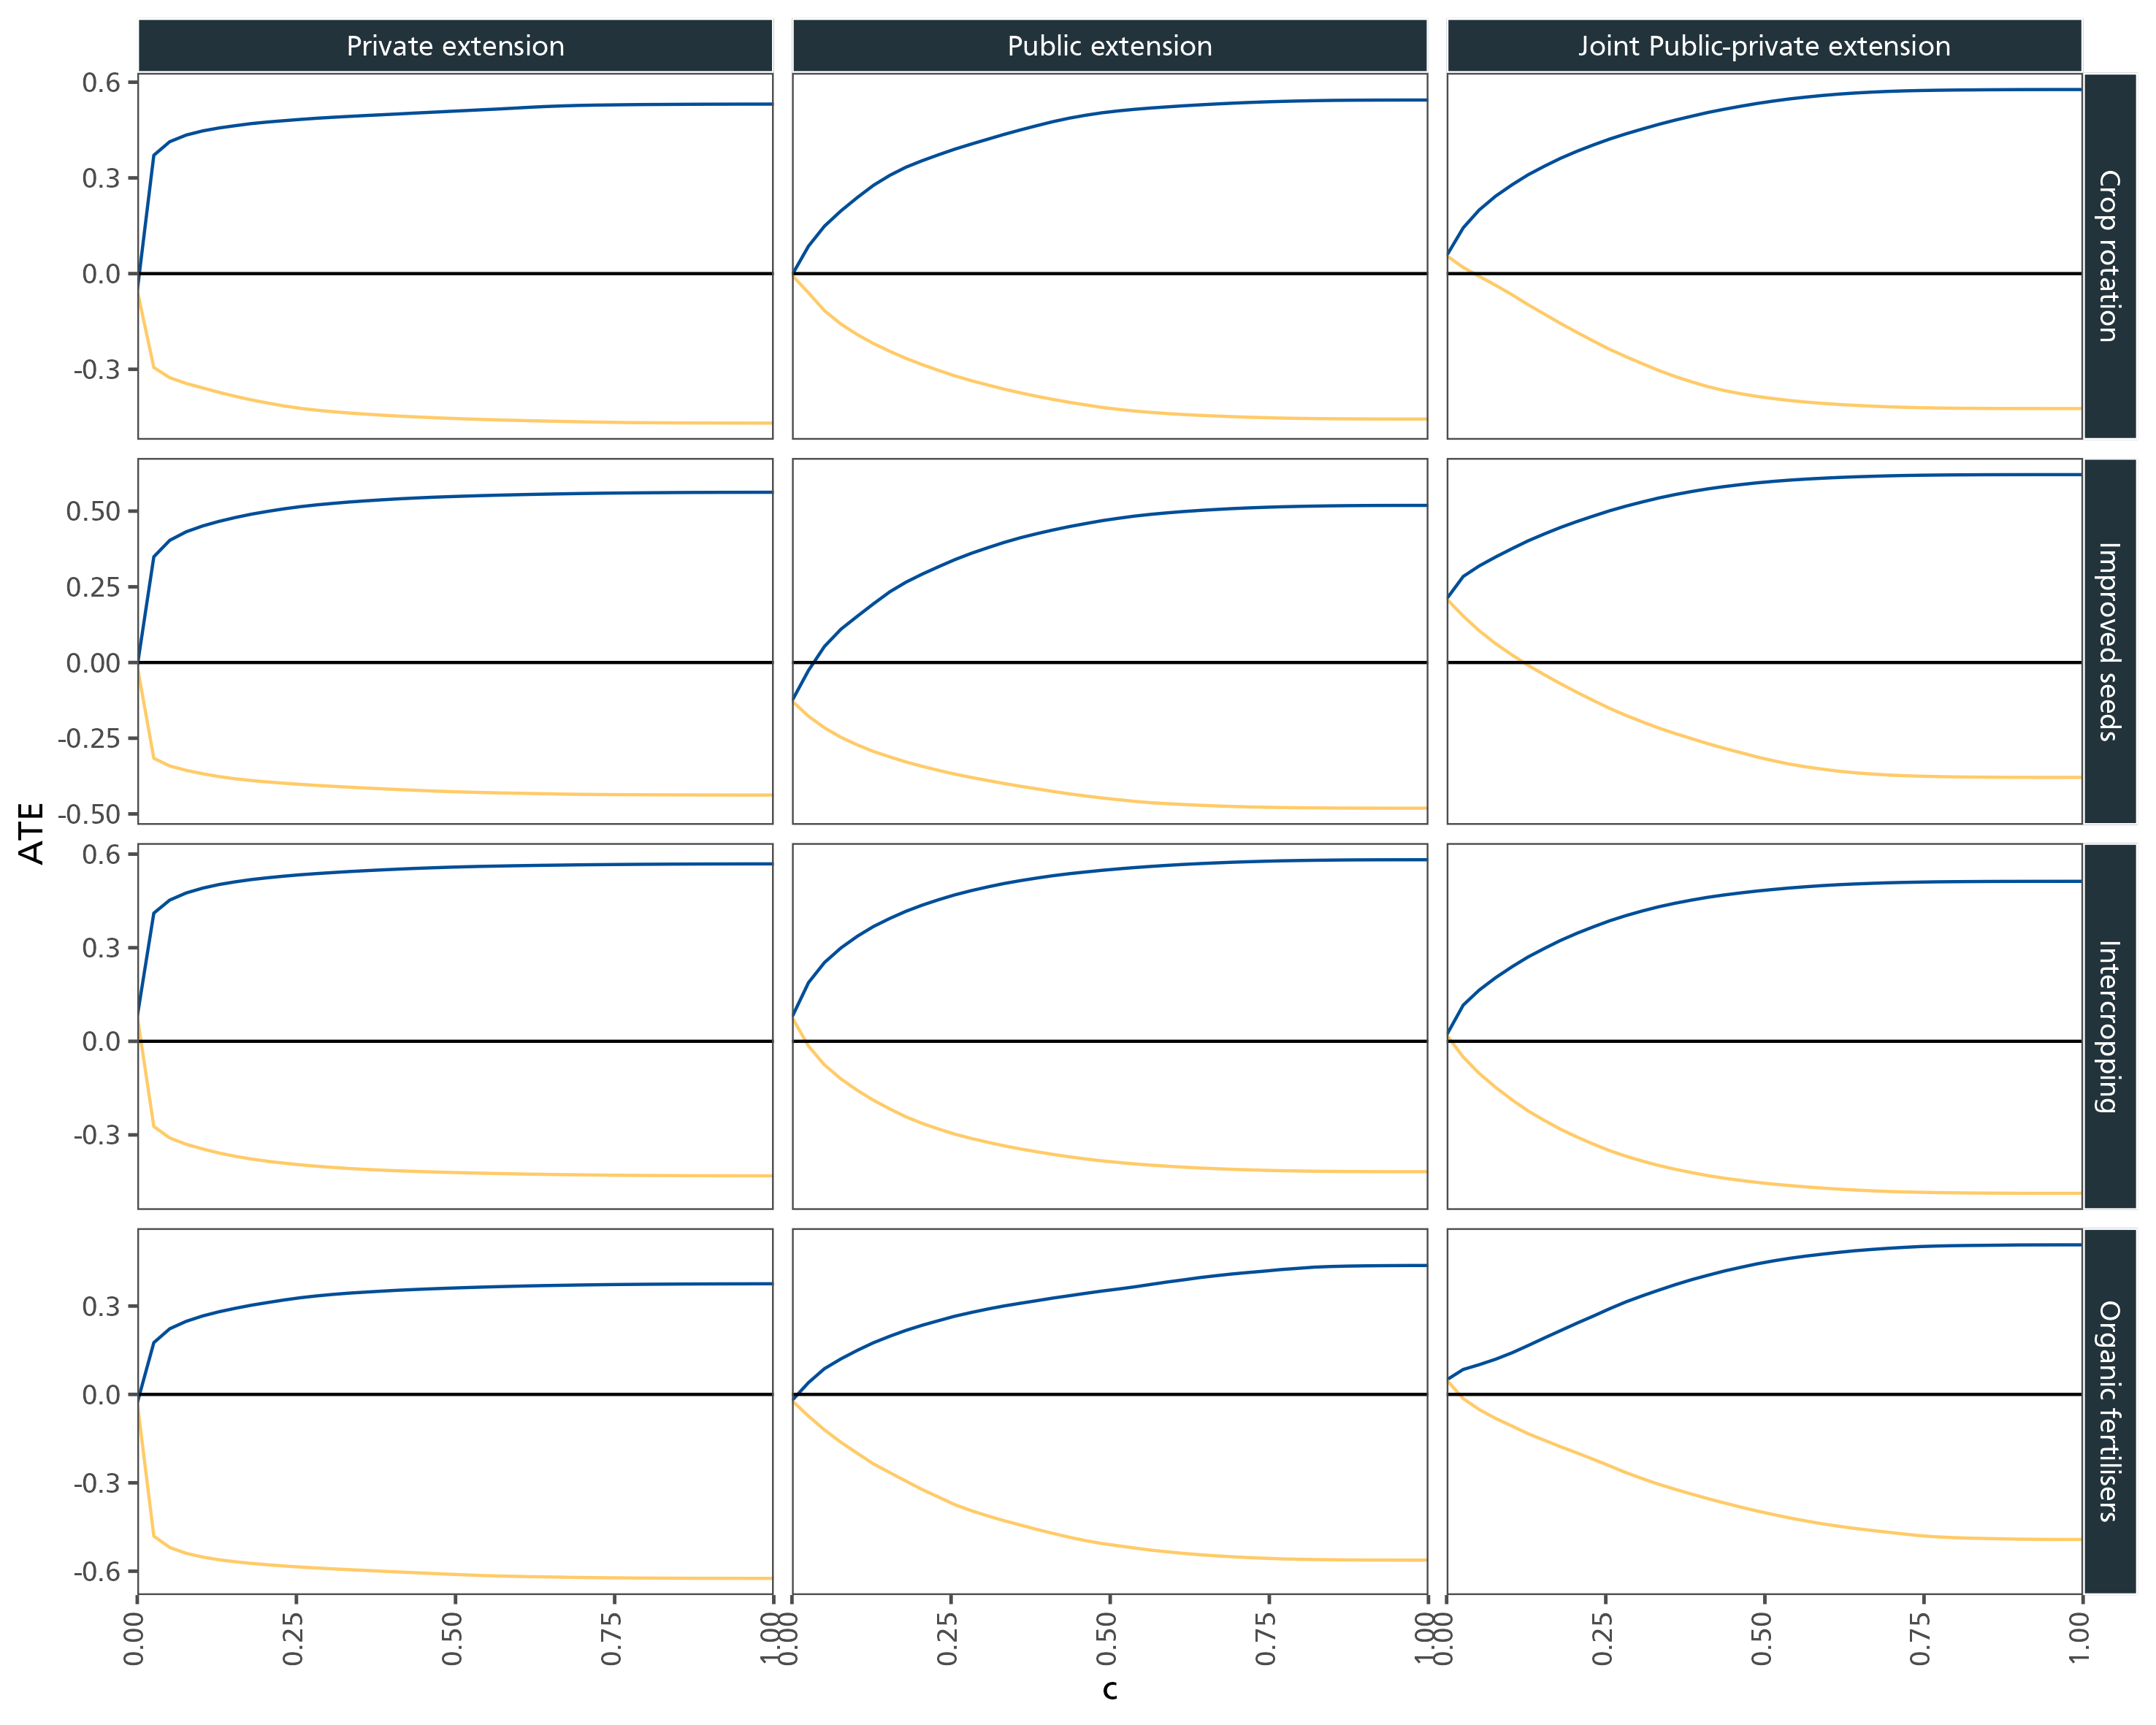
\includegraphics[width=1\textwidth]{Imbens_sensetivity.png}
\caption{Treatment effects sensitivity (Bounds on the ATE)}
\end{figure}

\pagebreak
\newpage

\begin{figure}[htbp]
\centering
\includegraphics[width=1\textwidth]{figures/sm_breakdown.png}
\caption{Regression sensitivity analysis (DMP 2022), breakdown}
\end{figure}

\pagebreak
\newpage

\begin{figure}[htbp]
\centering
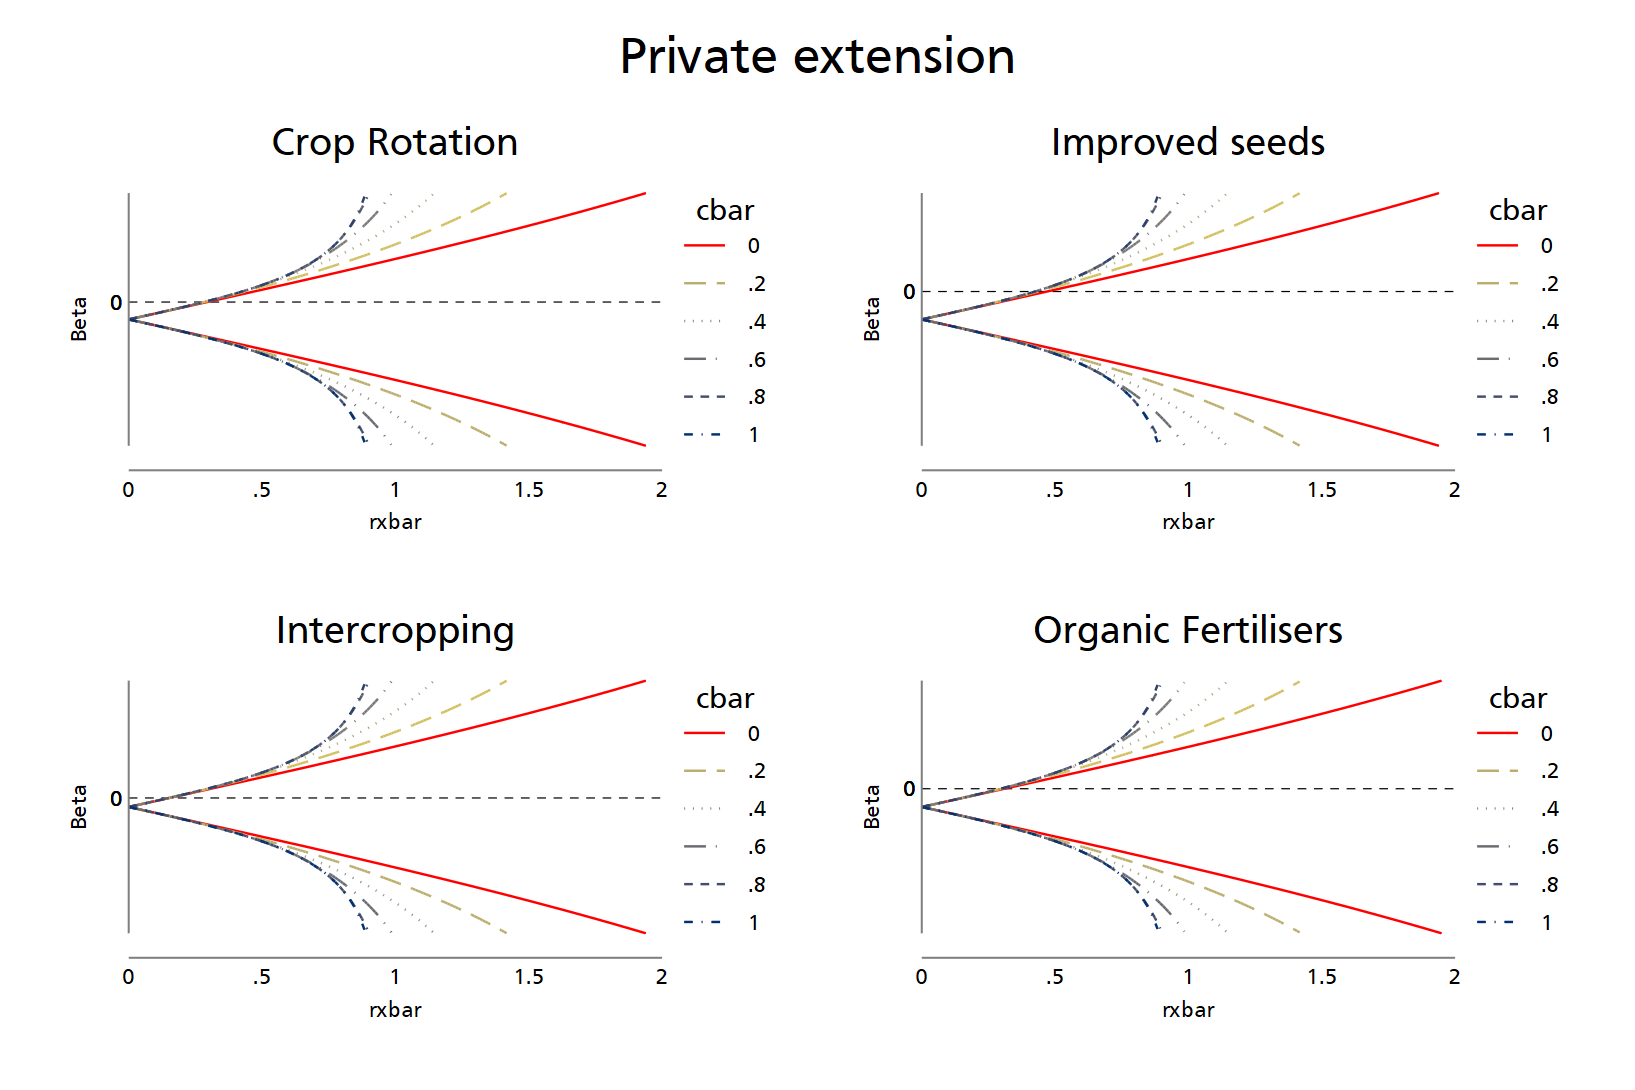
\includegraphics[width=1\textwidth]{figures/combined_private.png}
\caption{Selection and coefficent stability following the DMP 2022 (Private extension)}
\caption*{Note: The figure shows the sensitivity analysis conducted following Diegert et al. (2022). It presents the bounds derived from the estimated coefficients in the full model for private extension including all control variables as specified in Diegert et al. (2022). The coefficient values (rxbar) indicate the magnitude of selection on unobservables relative to observables that would be required to nullify the results of the study. Different line patterns within the figure represent different assumptions of endogeneity between the included controls and the omitted variables (cbar). In particular, the dotted line represents the most stringent scenario, assuming full endogeneity. For example,  the point of intersection at 0.28 from crop rotation implies that the baseline results are statistically significant and different from zero, provided that the selection on the unobservables does not exceed 28\% of the selection on the observables. The interesection point for improved seed, intercropping and organic fertilizer are 0.42, 0.15, 0.295 respectivelly.}
\end{figure}

\pagebreak
\newpage

\begin{figure}[htbp]
\centering
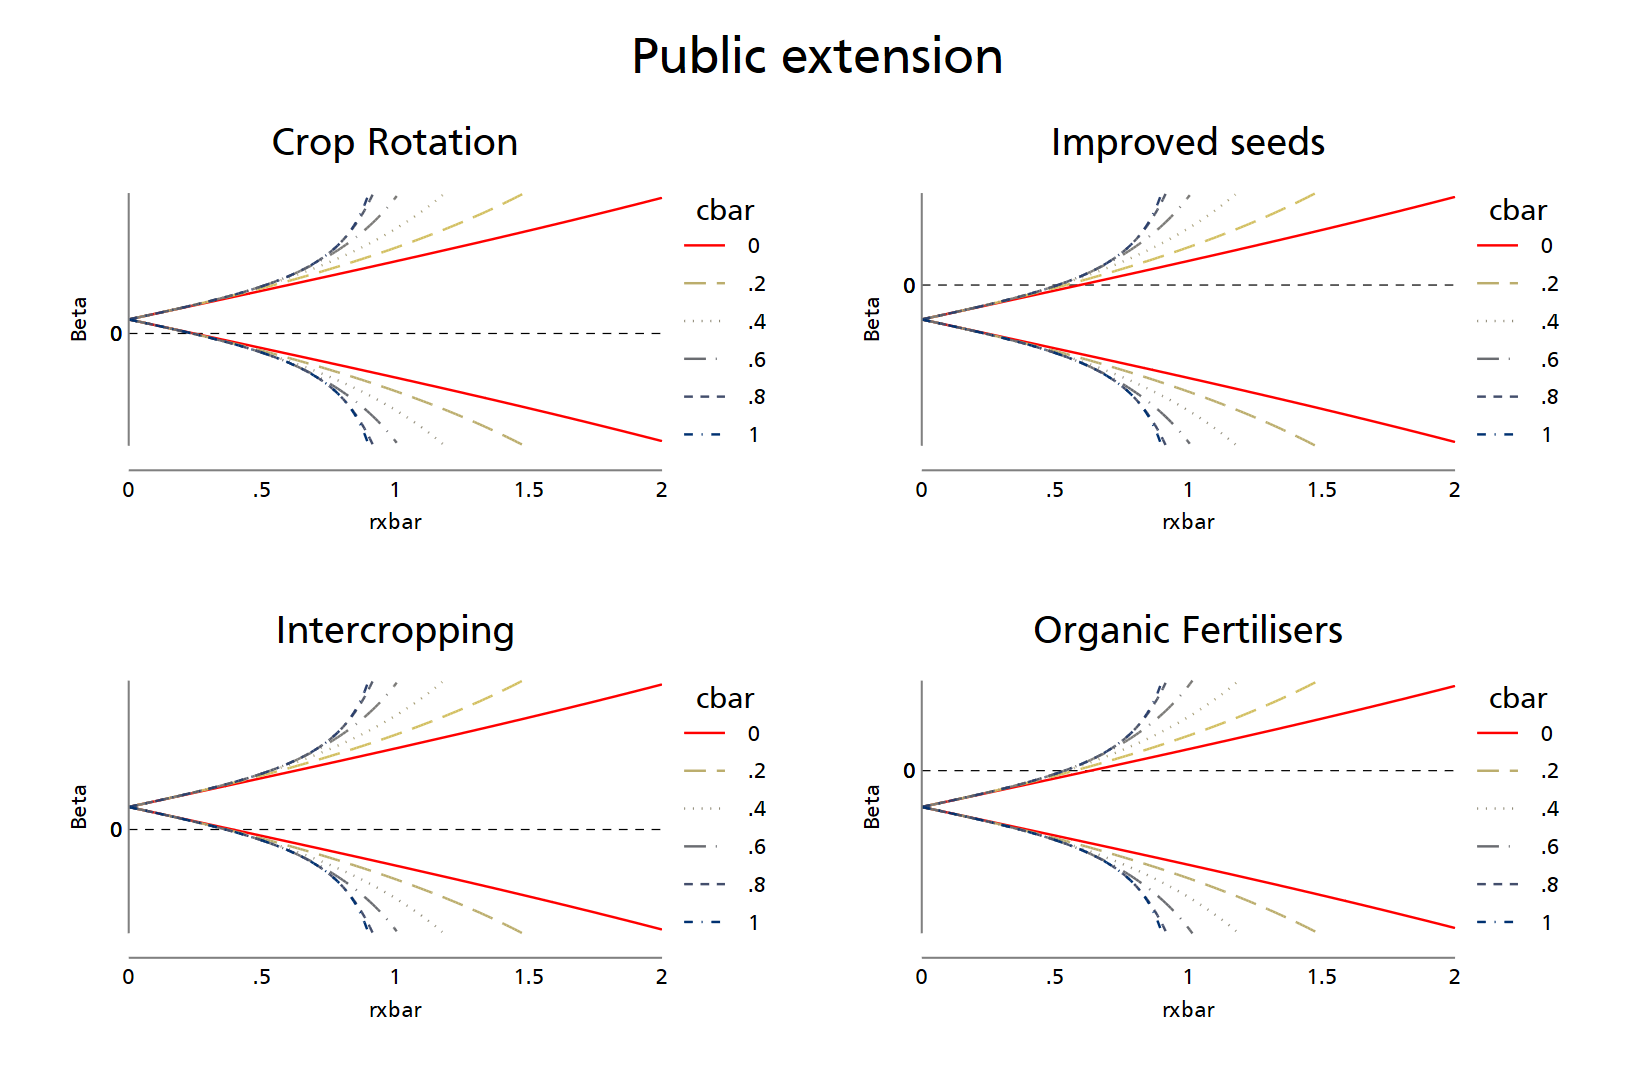
\includegraphics[width=1\textwidth]{figures/combined_public.png}
\caption{Selection and coefficent stability following the DMP 2022 (Public extension)}
\caption*{Note: The figure shows the sensitivity analysis conducted following Diegert et al. (2022). It presents the bounds derived from the estimated coefficients in the full model for public extension including all control variables as specified in Diegert et al. (2022). The coefficient values (rxbar) indicate the magnitude of selection on unobservables relative to observables that would be required to nullify the results of the study. Different line patterns within the figure represent different assumptions of endogeneity between the included controls and the omitted variables (cbar). In particular, the dotted line represents the most stringent scenario, assuming full endogeneity. For example,  the point of intersection at 0.239 from crop rotation implies that the baseline results are statistically significant and different from zero, provided that the selection on the unobservables does not exceed 23.9\% of the selection on the observables. The interesection point for improved seed, intercropping and organic fertilizer are 0.51, 0.364, 0.535 respectivelly.}
\end{figure}

\pagebreak
\newpage

\begin{figure}[htbp]
\centering
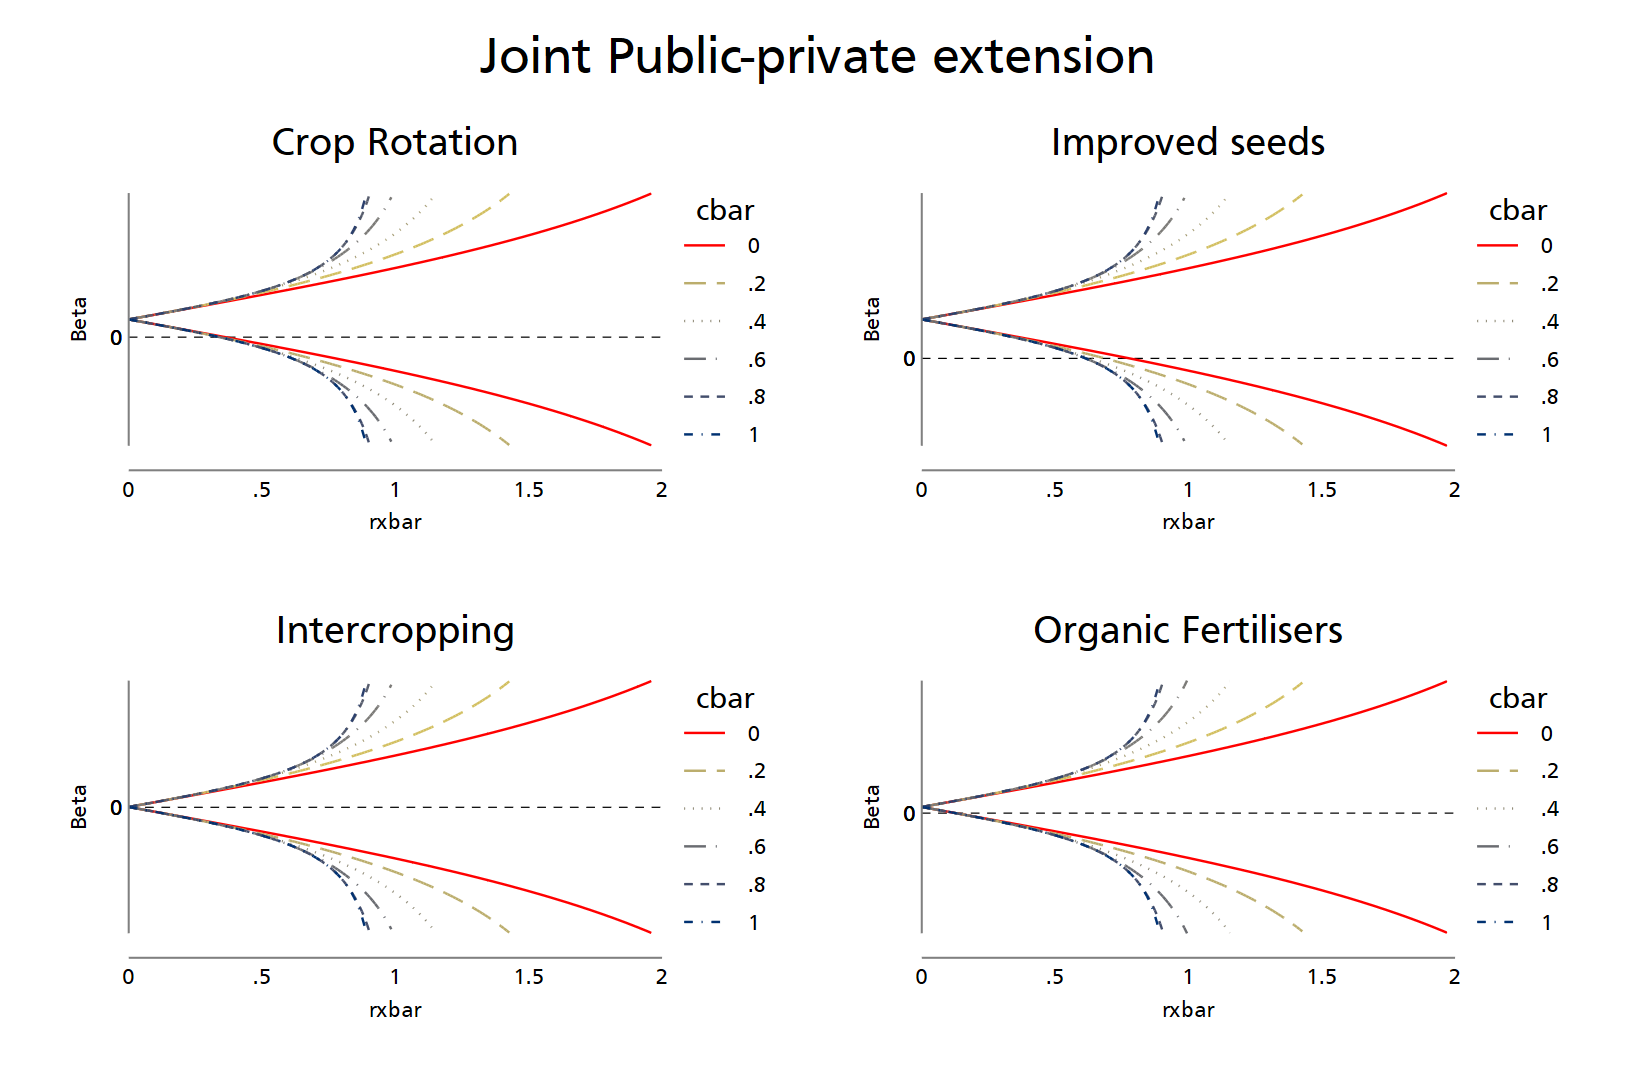
\includegraphics[width=1\textwidth]{figures/combined_joint.png}
\caption{Selection and coefficent stability following the DMP 2022 (Joint Public-private extension)}
\caption*{Note: The figure shows the sensitivity analysis conducted following Diegert et al. (2022). It presents the bounds derived from the estimated coefficients in the full model for joint private-public extension including all control variables as specified in Diegert et al. (2022). The coefficient values (rxbar) indicate the magnitude of selection on unobservables relative to observables that would be required to nullify the results of the study. Different line patterns within the figure represent different assumptions of endogeneity between the included controls and the omitted variables (cbar). In particular, the dotted line represents the most stringent scenario, assuming full endogeneity. For example,  the point of intersection at 0.341 from crop rotation implies that the baseline results are statistically significant and different from zero, provided that the selection on the unobservables does not exceed 34.1\% of the selection on the observables. The interesection point for improved seed, intercropping and organic fertilizer are 0.61, 0.07, 0.127 respectivelly.}
\end{figure}

\pagebreak
\newpage

\begingroup\fontsize{7}{9}\selectfont

\begin{longtable}[t]{lrrrr}
\caption{\label{tab:unnamed-chunk-9}Hausman Taylor estimation}\\
\toprule
Variables & Crop rotation & Improved seeds & Intercropping & Organic fertilisers\\
\midrule
\endfirsthead
\caption[]{\label{tab:unnamed-chunk-9}Hausman Taylor estimation \textit{(continued)}}\\
\toprule
Variables & Crop rotation & Improved seeds & Intercropping & Organic fertilisers\\
\midrule
\endhead

\endfoot
\bottomrule
\endlastfoot
Private extension & 0.040 & \textbf{0.077***} & \textbf{0.165***} & -0.048\\
 & (0.025) & (0.028) & (0.039) & (0.036)\\
Public extension & 0.014 & 0.025 & \textbf{0.174***} & -0.012\\
 & (0.022) & (0.021) & (0.025) & (0.016)\\
Joint Public-private extension & \textbf{0.127***} & \textbf{0.177***} & \textbf{0.157***} & \textbf{0.035**}\\
 & (0.019) & (0.021) & (0.022) & (0.016)\\
Age of household head (years) & \textbf{-0.001**} & 0.000 & -0.001 & 0.000\\
 & (0.000) & (0.000) & (0.001) & (0.000)\\
Household size (number of persons) & 0.002 & \textbf{-0.002*} & \textbf{0.006***} & \textbf{-0.005***}\\
 & (0.001) & (0.001) & (0.001) & (0.001)\\
Distance to the nearest urban market (km) & \textbf{0.002***} & \textbf{-0.002***} & \textbf{-0.001*} & \textbf{0.002***}\\
 & (0.000) & (0.001) & (0.001) & (0.001)\\
Distance the nearest village market (km) & \textbf{-0.010***} & \textbf{0.005***} & \textbf{-0.006***} & \textbf{-0.003**}\\
 & (0.002) & (0.001) & (0.002) & (0.001)\\
Cooperative membership (dummy) & \textbf{0.040**} & \textbf{0.030*} & 0.014 & \textbf{0.030**}\\
 & (0.016) & (0.016) & (0.021) & (0.013)\\
Labor cost (USD/ha) & 0.000 & \textbf{0.001***} & -0.000 & \textbf{0.001***}\\
 & (0.000) & (0.000) & (0.000) & (0.000)\\
Groundnut area (ha) & \textbf{0.036***} & \textbf{0.019***} & \textbf{0.017***} & \textbf{0.045***}\\
 & (0.005) & (0.005) & (0.006) & (0.005)\\
Off-farm income (dummy) & 0.011 & \textbf{0.047*} & 0.002 & \textbf{-0.062***}\\
 & (0.022) & (0.027) & (0.029) & (0.021)\\
Dependency ratio & -0.001 & -0.002 & \textbf{0.016***} & \textbf{0.017***}\\
 & (0.005) & (0.005) & (0.006) & (0.004)\\
Clay soil (dummy) & 0.033 & -0.012 & 0.020 & 0.006\\
 & (0.021) & (0.020) & (0.025) & (0.018)\\
Sandy-clay soil (dummy) & 0.023 & -0.010 & 0.023 & \textbf{0.033**}\\
 & (0.016) & (0.016) & (0.020) & (0.015)\\
Silty soil (dummy) & \textbf{0.035*} & 0.002 & 0.022 & 0.012\\
 & (0.020) & (0.020) & (0.025) & (0.018)\\
Sex of household head (dummy, male=1) & 0.027 & \textbf{0.077***} & \textbf{-0.056*} & -0.006\\
 & (0.025) & (0.023) & (0.031) & (0.022)\\
Education level (Number of years) & -0.001 & \textbf{0.003**} & -0.003 & -0.001\\
 & (0.002) & (0.002) & (0.002) & (0.001)\\
Constant & -0.025 & \textbf{0.422***} & \textbf{0.293***} & \textbf{0.842***}\\
 & (0.051) & (0.050) & (0.071) & (0.039)\\
\midrule
Observations & 8,604 & 8,604 & 8,604 & 8,604\\
Number of id & 2,868 & 2,868 & 2,868 & 2,868\\
Additional controls & Yes & Yes & Yes & Yes\\
District FE & Yes & Yes & Yes & Yes\\
Year FE & Yes & Yes & Yes & Yes\\
\midrule
Robust standard errors in parentheses &  &  &  & \\
*** p<0.01, ** p<0.05, * p<0.1 &  &  &  & \\*
\end{longtable}
\endgroup{}

\newpage

\begingroup\fontsize{7}{9}\selectfont

\begin{longtable}[t]{lrrrr}
\caption{\label{tab:unnamed-chunk-10}Attrition bias check}\\
\toprule
Variables & Overall & Ghana & Mali & Nigeria\\
\midrule
\endfirsthead
\caption[]{\label{tab:unnamed-chunk-10}Attrition bias check \textit{(continued)}}\\
\toprule
Variables & Overall & Ghana & Mali & Nigeria\\
\midrule
\endhead

\endfoot
\bottomrule
\endlastfoot
Sex of household head & 0.0597 & 0.0348 & 0.133 & 0.191\\
 & (0.159) & (0.234) & (0.339) & (0.433)\\
Age of household head (years) & 0.00488 & -0.00385 & 0.00724 & 0.00255\\
 & (0.00397) & (0.00996) & (0.00618) & (0.00687)\\
Number of years at school without repetition & -0.00311 & -0.0114 & -0.00182 & 0.0124\\
 & (0.00997) & (0.0241) & (0.0272) & (0.0131)\\
Number of years in groundnut production as independent household head & -0.00214 & 0.00415 & -0.00854 & 0.00380\\
 & (0.00423) & (0.0114) & (0.00673) & (0.00713)\\
Number of people in the household & 0.000260 & 0.0112 & -0.00362 & -0.00254\\
 & (0.00438) & (0.0190) & (0.00625) & (0.0120)\\
dependency ratio & -0.0379 & -0.0422 & 0.0500 & -0.0526\\
 & (0.0286) & (0.0732) & (0.0579) & (0.0398)\\
Have you or other members of your household received cash credit for groundnut d & 0.266 & 0.352 & 0.337 & 0.0955\\
 & (0.165) & (0.600) & (0.226) & (0.294)\\
Have you or other members of your household received credit in kind for groundnu & -0.117 &  & 0.173 & -0.0908\\
 & (0.146) &  & (0.237) & (0.204)\\
Log household distance to urban market & 0.0412 & 0.0655 & \textbf{0.115*} & -0.0110\\
 & (0.0393) & (0.160) & (0.0626) & (0.0589)\\
off-farm income & -0.148 &  & 0.391 & -0.0495\\
 & (0.128) &  & (0.347) & (0.149)\\
Constant & \textbf{-1.850***} & \textbf{-1.497***} & \textbf{-2.194***} & \textbf{-1.988***}\\
 & (0.249) & (0.576) & (0.462) & (0.551)\\
Observations & 3,040 & 517 & 900 & 1,600\\
Standard errors in parentheses &  &  &  & \\
*** p<0.01, ** p<0.05, * p<0.1 &  &  &  & \\*
\end{longtable}
\endgroup{}

\end{document}
